\documentclass[10pt,letterpaper]{article}
\usepackage[margin=1in,bottom=1.05in]{geometry}
\usepackage{amsmath,amssymb,amsthm,mathtools}
\usepackage{graphicx}
\usepackage{booktabs,array,longtable}
\usepackage{xcolor}
\usepackage[numbers,sort&compress]{natbib}
\usepackage[hidelinks]{hyperref}
\usepackage{xurl}
\usepackage{caption}
\captionsetup{skip=3pt}
\usepackage[compact]{titlesec}
\titlespacing*{\section}{0pt}{8pt}{4pt}
\titlespacing*{\subsection}{0pt}{6pt}{3pt}
\titlespacing*{\paragraph}{0pt}{4pt}{1em}
\setlength{\textfloatsep}{8pt plus 2pt minus 2pt}
\setlength{\floatsep}{6pt plus 2pt minus 2pt}
\setlength{\intextsep}{6pt plus 2pt minus 2pt}
\setlength{\emergencystretch}{2em}

\newtheorem{proposition}{Proposition}
\newtheorem{theorem}[proposition]{Theorem}
\newtheorem{lemma}{Lemma}
\newtheorem{corollary}{Corollary}
\theoremstyle{definition}
\newtheorem{definition}{Definition}
\theoremstyle{remark}
\newtheorem{remark}{Remark}

\newcommand{\E}{\mathbb{E}}
\newcommand{\Var}{\mathrm{Var}}
\newcommand{\Cov}{\mathrm{Cov}}
\newcommand{\ES}{\mathrm{ES}}
\newcommand{\method}{\textnormal{\textsc{Ligature}}}

\title{\textsc{Ligature}: Generative Inference of Spatial Molecular Organization from Histology}
\author{Adhiban Arulselvan\\[2pt]
{\normalsize Computer Science and Artificial Intelligence Laboratory (CSAIL)}\\
{\normalsize Massachusetts Institute of Technology}\\
{\normalsize\texttt{adhiban@mit.edu}}}
\date{}
\renewcommand{\abstractname}{\normalsize Abstract}

\newcommand{\RefMSE}{0.88}
\newcommand{\SeedMSEMean}{0.92}
\newcommand{\SeedMSESD}{0.02}
\newcommand{\SeedMSEMin}{0.898}
\newcommand{\SeedMSEMax}{0.945}
\newcommand{\RefCoverage}{74.2}
\newcommand{\SeedCoverageMean}{72.9}
\newcommand{\SeedCoverageSD}{0.9}
\newcommand{\SeedCoverageMin}{72.1}
\newcommand{\SeedCoverageMax}{73.9}
\newcommand{\IndependentCoverage}{49.4}
\newcommand{\NoPatientCoverage}{49.8}
\newcommand{\CurrentNoPatientCoverage}{49.2}
\newcommand{\RefCRPS}{0.0274}
\newcommand{\GaussianCRPS}{0.0326}
\newcommand{\CRPSReduction}{16.1}
\newcommand{\CurrentCellOnlyMSE}{1.33}
\newcommand{\OldCellOnlyMSE}{2.40}
\newcommand{\CurrentNoFieldsMSE}{1.00}
\newcommand{\OldNoFieldsMSE}{1.03}
\newcommand{\SeedAllMSE}{0.91}
\newcommand{\SeedCrossMSE}{0.95}
\newcommand{\SeedSameMSE}{0.61}
\newcommand{\DirectAllMSE}{0.88}
\newcommand{\DirectCrossMSE}{0.92}
\newcommand{\DirectSameMSE}{0.64}
\newcommand{\AggregateCRPS}{0.0277}
\newcommand{\AggregateCoverage}{73.3}

\newcommand{\ControlRegions}{3,322}
\newcommand{\ControlRemovedPercent}{20.3}
\newcommand{\ControlInitialPairs}{1,938,513}
\newcommand{\ControlRetainedPairs}{1,545,721}
\newcommand{\ControlRemovedPairs}{392,792}
\newcommand{\ControlMSE}{0.72}
\newcommand{\ControlLower}{0.62}
\newcommand{\ControlUpper}{1.07}
\newcommand{\ControlPluginBias}{-53}
\newcommand{\ControlJointBias}{+6}

\newcommand{\BaseRefConstAll}{0.98}
\newcommand{\BaseRefConstCross}{1.02}
\newcommand{\BaseRefConstSame}{0.69}
\newcommand{\BaseRefConstRho}{0.44}
\newcommand{\BaseRefConstBiasAll}{+2}
\newcommand{\BaseRefConstBiasSame}{+2}
\newcommand{\BaseRefDiffAll}{-0.10}
\newcommand{\BaseRefDiffAllLo}{-0.25}
\newcommand{\BaseRefDiffAllHi}{-0.02}
\newcommand{\BaseRefDiffSame}{-0.09}
\newcommand{\BaseRefDiffSameLo}{-0.46}
\newcommand{\BaseRefDiffSameHi}{0.002}
\newcommand{\BaseLungConstAll}{0.96}
\newcommand{\BaseLungConstCross}{1.01}
\newcommand{\BaseLungConstSame}{0.64}
\newcommand{\BaseLungConstRho}{0.35}
\newcommand{\BaseLungConstBiasAll}{0}
\newcommand{\BaseLungConstBiasSame}{+1}
\newcommand{\BaseLungDiffAll}{-0.13}
\newcommand{\BaseLungDiffAllLo}{-1.05}
\newcommand{\BaseLungDiffAllHi}{-0.09}
\newcommand{\BaseLungDiffSame}{-0.15}
\newcommand{\BaseLungDiffSameLo}{-1.05}
\newcommand{\BaseLungDiffSameHi}{-0.06}
\newcommand{\BaseRefLigRho}{0.53}
\newcommand{\BaseNoImageScore}{6.78}
\newcommand{\BaseConstScore}{5.58}
\newcommand{\BaseConstSameScore}{5.39}
\newcommand{\BaseRidgeScore}{5.80}
\newcommand{\BaseRidgeAll}{1.03}
\newcommand{\BaseRidgeSame}{0.71}
\newcommand{\BaseConstAll}{1.01}
\newcommand{\BaseConstSame}{0.73}
\newcommand{\BaseLigConstScore}{-0.60}
\newcommand{\BaseLigConstScoreLo}{-0.91}
\newcommand{\BaseLigConstScoreHi}{-0.27}
\newcommand{\BaseLigConstSameScore}{-0.23}
\newcommand{\BaseLigConstSameScoreLo}{-0.93}
\newcommand{\BaseLigConstSameScoreHi}{0.45}
\newcommand{\BaseDirConstScore}{-0.01}
\newcommand{\BaseDirConstScoreLo}{-0.21}
\newcommand{\BaseDirConstScoreHi}{0.22}
\newcommand{\BaseLigRidgeScore}{-0.82}
\newcommand{\BaseLigRidgeScoreLo}{-1.13}
\newcommand{\BaseLigRidgeScoreHi}{-0.47}
\newcommand{\BaseLigRidgeSameScore}{-0.40}
\newcommand{\BaseLigRidgeSameScoreLo}{-0.98}
\newcommand{\BaseLigRidgeSameScoreHi}{0.24}
\newcommand{\BaseLigConstMSE}{-0.05}
\newcommand{\BaseLigConstMSELo}{-0.18}
\newcommand{\BaseLigConstMSEHi}{0.02}
\newcommand{\BaseLigConstSameMSE}{-0.07}
\newcommand{\BaseLigConstSameMSELo}{-0.20}
\newcommand{\BaseLigConstSameMSEHi}{0.06}
\newcommand{\BaseLigRidgeMSE}{-0.07}
\newcommand{\BaseLigRidgeMSELo}{-0.19}
\newcommand{\BaseLigRidgeMSEHi}{0.01}
\newcommand{\BaseLigRidgeSameMSE}{-0.04}
\newcommand{\BaseLigRidgeSameMSELo}{-0.12}
\newcommand{\BaseLigRidgeSameMSEHi}{0.11}
\newcommand{\BaseInsampleAll}{0.93}
\newcommand{\BaseInsampleSame}{0.68}
\newcommand{\BaseInsampleScore}{5.57}
\newcommand{\BaseLigInsampleScore}{-0.59}
\newcommand{\BaseLigInsampleScoreLo}{-0.92}
\newcommand{\BaseLigInsampleScoreHi}{-0.22}
\newcommand{\BaseSelectionAll}{1.50}
\newcommand{\BaseFixedAllLo}{0.93}
\newcommand{\BaseFixedAllHi}{0.94}
\newcommand{\BaseFixedSameLo}{0.63}
\newcommand{\BaseFixedSameHi}{0.68}
\newcommand{\BaseFixedMinScore}{5.61}
\newcommand{\BaseFixedWorstAll}{1.56}
\newcommand{\BaseFixedMinSameScore}{5.13}
\newcommand{\BaseLigFixedScore}{-0.62}
\newcommand{\BaseLigFixedScoreLo}{-0.92}
\newcommand{\BaseLigFixedScoreHi}{-0.32}
\newcommand{\BaseMoranNoImage}{0.42}
\newcommand{\BaseMoranConst}{0.31}
\newcommand{\BaseMoranNoImageScore}{5.08}
\newcommand{\BaseMoranConstScore}{5.88}
\newcommand{\BaseGearyNoImage}{0.52}
\newcommand{\BaseGearyConst}{0.38}
\newcommand{\BaseGearyNoImageScore}{5.35}
\newcommand{\BaseGearyConstScore}{4.86}
\newcommand{\BaseIndDirectBias}{-16}
\newcommand{\BaseIndDirectBiasSame}{-26}
\newcommand{\BaseIndLigBias}{-6}
\newcommand{\BaseIndLigBiasSame}{-2}
\newcommand{\BaseIndConstBias}{+5}
\newcommand{\BaseIndConstBiasSame}{+3}
\newcommand{\BaseIndRidgeBias}{-9}
\newcommand{\BaseIndRidgeBiasSame}{-9}


\begin{document}
\hypersetup{pageanchor=false}
\maketitle

\begin{abstract}\normalsize
Virtual stains predict molecular profiles from hematoxylin and eosin (H\&E) images, but their per-cell objectives do not target the relationships underlying molecular clustering and immune co-localization. Given cell segmentations, we formulate spatial molecular inference as learning residual dependence targeted to downstream statistics. Conditional-mean plug-in estimates of bilinear statistics omit cross-cell residual covariance; even exact per-cell marginals leave their expectations unidentified, with semidefinite bounds for Gaussian marginals. \method{} implements this formulation around a frozen virtual stain, using morphology-conditioned multiscale Gaussian fields and region- and patient-level latent variables to generate joint molecular samples. Strictly proper scores on region- and patient-level spatial statistics align training with downstream analyses. In a reference patient-disjoint evaluation of 40 colorectal cancer patients with paired H\&E and 16-plex immunofluorescence, median attenuation of non-negligible cohort means decreased from 34\% to 6\%. Clustering mean squared error in training-standardized coordinates fell by 40\% relative to the stain (39\% over four runs). In an exploratory comparison under independent calibration across three seeds, overall interval score was 10.6\% below a matched direct graph's at approximately 90\% coverage; clustering-interval and point-error comparisons were inconclusive. Frozen samples supported gated contacts excluded from training, with 30\% lower error than a quantile-matched stain, although adapted predictors performed better on new autocorrelation queries. In a separate 19-patient lung Xenium evaluation, overall and clustering error decreased by 16\% and 52\% relative to its stain. These results support dependence modeling for spatial inference, with gains dependent on the query and intensity scale; interval calibration requires separate molecular measurements.
\end{abstract}
\thispagestyle{empty}
\newpage
\setcounter{page}{1}
\hypersetup{pageanchor=true}

\section{Introduction}

Spatial tissue analyses quantify how molecular states vary across neighboring cells: immune infiltration of tumor nests, macrophage--checkpoint contacts, and clustering of proliferating or lineage-defined cells. Inferring these quantities from routine hematoxylin and eosin (H\&E) requires predictions for region- and patient-level statistics. Analyses may introduce new gates, neighborhoods and distances after training. Virtual multiplexing models already predict molecular markers from H\&E at population scale \citep{gigatime2025,rosie2025,hex2026}; GigaTIME, for example, generated virtual immunofluorescence for 14,256 patients \citep{gigatime2025}. We target spatial-statistic estimates and probabilistic forecasts from these cell predictions.

We introduce \method{}, a statistic-scored generative residual model. It keeps a frozen virtual stain as its mean and fits an image-conditioned distribution over the residuals of all cells jointly. A cell-graph transformer reads the tissue and parameterizes loadings on spatial Gaussian fields, cell noise, and region and patient latents. Training scores cell markers, spatial moments and patient summaries with the continuous ranked probability score (CRPS), so spatial dependence is fitted against the analyses it must support. At inference, the same joint samples supply estimates and predictive distributions for both the scored statistics and additional nonlinear queries. Query-specific calibration on separate measured patients provides marginal prediction intervals.

The statistical rationale connects this design to the target quantities. For a bilinear statistic, the gap between its conditional expectation and the plug-in of a per-cell-optimal predictor is a weighted residual covariance (Proposition~\ref{prop:bias}). Per-cell marginal laws leave this covariance unidentified; we characterize the resulting range by certified semidefinite computations (Proposition~\ref{prop:nonid}). Scoring spatial statistics instead specifies their conditional-law targets under a correctly specified generator class (Propositions~\ref{prop:proper}--\ref{prop:ident}), while likelihood uses different covariance weights under misspecification (Proposition~\ref{prop:alloc}). Generated maps are realizations of the fitted model; our validation concerns their spatial-statistic forecasts, without claiming recovery of an individual tissue's unique unobserved molecular configuration.

Our contributions are: (i) a joint residual generator and analysis-directed training procedure that connect frozen virtual stains to spatial inference, with shared sampling across regions and patient-disjoint statistic-level calibration; (ii) statistical rationale and computable identification bounds for the dependence targeted by the procedure; and (iii) a patient-held-out evaluation across six stains, two cohorts and assay modalities, direct and probabilistic baselines, systematic ablations, and nonlinear statistics absent from training.

\section{Related work}

\paragraph{Virtual multiplex from histology.} ROSIE \citep{rosie2025}, HEX \citep{hex2026}, GigaTIME \citep{gigatime2025}, generative image translators \citep{virtualmultiplexer} and diffusion-based multimodal histopathology models such as MuPD \citep{mupd2026} predict protein maps from H\&E; related models represent measured panels (VirTues \citep{virtues2026}), impute missing markers (CytoVI \citep{cytovi2026}) or choose markers to measure (ECHO-k \citep{echok2026}). Per-cell/pixel and downstream evaluations do not establish the spatial-statistic law. Concurrently, CellPlex \citep{cellplex2026} benchmarks per-cell protein prediction from H\&E across seven cohorts, including ORION-CRC; our target is the spatial-statistic law computed from molecular predictions, rather than per-cell prediction accuracy.

\paragraph{Uncertainty for imputed spatial omics.} TISSUE \citep{tissue2024} gives conformal per-cell intervals for imputed spatial transcriptomes and propagates them to downstream tests by multiple imputation, and SpatialNP \citep{spatialnp2026} applies neural processes to probabilistic multiplexed tissue imaging. Per-unit marginals alone do not specify cross-cell statistics (Proposition~\ref{prop:nonid}). Bounds on dependence given marginals are classical (Fr\'echet--Hoeffding bounds, statistical matching); the proposition specializes the Gaussian-marginal case to spatial statistics and makes it computable and certified at tissue scale.

\paragraph{Prediction-powered and design-based correction.} Prediction-powered inference \citep{ppi2023,activeinference2024}, semi-supervised U-statistics \citep{kim2024ssu}, and spatially dependent PPI \citep{ppispatial2026} combine model predictions with a labeled subsample for valid inference on population-level targets. \method{} predicts for individual patients conditional on supplied cell geometry; its predictions can serve as inputs to such estimators.

\paragraph{Proper scoring rules and generative distributional regression.} Energy-score training of noise-injected generators (engression \citep{engression2024}) and CRPS-trained generative weather ensembles \citep{fgn2025} learn conditional distributions without likelihoods. We bring this principle to tissue and score the statistics analyzed downstream; as in weather forecasting \citep{pinson2013,scheuerer2015}, a single high-dimensional energy score appeared insufficient in a preliminary run (Appendix~\ref{app:impl}).

\section{Method}
\label{sec:method}

\paragraph{Task and interface.} Training uses paired H\&E and molecular measurements on segmented regions. Inputs at deployment are H\&E cell features, cell positions and shape descriptors from a supplied segmentation, and a frozen stain; outputs are joint molecular draws and statistics computed on them. Primary evaluations use assay segmentations; a separate H\&E-derived proxy control changes both geometry and target definition (Appendix~\ref{app:querybench}). Interval calibration for new queries uses their values on a separate measured patient set. This evaluates statistical inference conditional on the supplied segmentation.

A region (crop) of a section contains cells $i=1,\dots,n$ at positions $x_i$ with context $H$ collecting H\&E features and supplied geometry, and molecular vector $Y_i\in\mathbb{R}^p$ (standardized log intensities). Write $d_{ij}=\lVert x_i-x_j\rVert$ and let $|E_w|$ denote the pair-count normalization for radial weight $w$. For markers $(a,b)$, a bilinear spatial statistic is
\begin{equation}
Q_{w,ab}(Y) = \frac{1}{|E_w|}\sum_{i\neq j} w(d_{ij})\,\tfrac12\,(Y_{ia}Y_{jb}+Y_{ib}Y_{ja}).
\end{equation}
Our primary contrast uses $w=\mathbf{1}\{d\le 25\,\mu\mathrm{m}\}$ normalized by its pair count minus $\mathbf{1}\{50<d\le75\,\mu\mathrm{m}\}$ normalized likewise. It compares nearby marker products with a distant within-region reference; for $a=b$ it measures same-marker clustering in training-standardized log intensities. Centering and scaling define the estimand. Original-log-intensity contrasts and Moran's $I$/Geary's $C$ provide complementary evaluations (Section~\ref{sec:unscored}). Patient-level statistics average crops with equal weight.

\begin{definition}[Spatial statistic vector]
For distance bins $B_1,\dots,B_K$, let $S(Y)$ collect the cell means, the binned symmetric second moments $G_{k,ab}=|E_k|^{-1}\sum_{i\ne j:\,d_{ij}\in B_k}\frac12(Y_{ia}Y_{jb}+Y_{ib}Y_{ja})$ for every bin $k$ and unordered pair $a\le b$, and the bin contrasts $G_{k,ab}-G_{k',ab}$.
\end{definition}

\paragraph{Generative model.} \method{} wraps a frozen per-cell virtual stain $f(H)\in\mathbb{R}^{n\times p}$ with an image-conditioned joint residual distribution. A model draw is
\begin{equation}\label{eq:model}
Y_i = f_i(H) + \sum_{\ell=1}^{4} A_{\ell}(H)_i\,\xi_{\ell,r(i)}(x_i) + B(H)_i\,\epsilon_i + C(H)_i\,\zeta_{r(i)} + D(H)_i\,\eta_g ,
\end{equation}
where $r(i)$ indexes cell $i$'s region, and $\xi_{\ell,r}$ are independent four-variate unit Gaussian random fields with squared-exponential correlation at length scales $\ell\in\{10,20,40,80\}\,\mu$m (approximated with 64 random Fourier features per field and region), $\epsilon_i$ is cell noise, $\zeta_r$ a region latent and $\eta_g$ a patient latent shared by all regions of patient $g$. The loading matrices $A_\ell,B,C,D\in\mathbb{R}^{p\times\cdot}$ are per-cell outputs of a cell-graph transformer, so that the within-patient residual covariance
$\Cov(Y_i,Y_j\mid H)=\mathbf{1}_{r(i)=r(j)}[\sum_\ell k_\ell(d_{ij})A_{\ell i}A_{\ell j}^\top+C_iC_j^\top]+\mathbf{1}_{i=j}B_iB_i^\top+D_iD_j^\top$
is positive semidefinite by construction, cross-marker, spatially structured, and morphology dependent (a linear model of coregionalization whose coefficients are read from the tissue). If $f=\mu$, Proposition~\ref{prop:bias} makes the plug-in bias of every bilinear statistic the corresponding weighted sum of these covariances. Write $X_{k,ab}(f,\delta)=G_{k,ab}(f+\delta)-G_{k,ab}(f)-G_{k,ab}(\delta)$ for the bilinear cross term. For mean error $\delta=\mu-f$, suppressing bin/marker subscripts, matching a binned statistic's mean gives $\Gamma(\hat\Sigma)=\Gamma(\Sigma)+G(\delta)+X(f,\delta)$: the generated covariance absorbs the stain's mean error and equals $\Sigma$ there only when $f=\mu$.

\begin{figure}[!t]
\centering
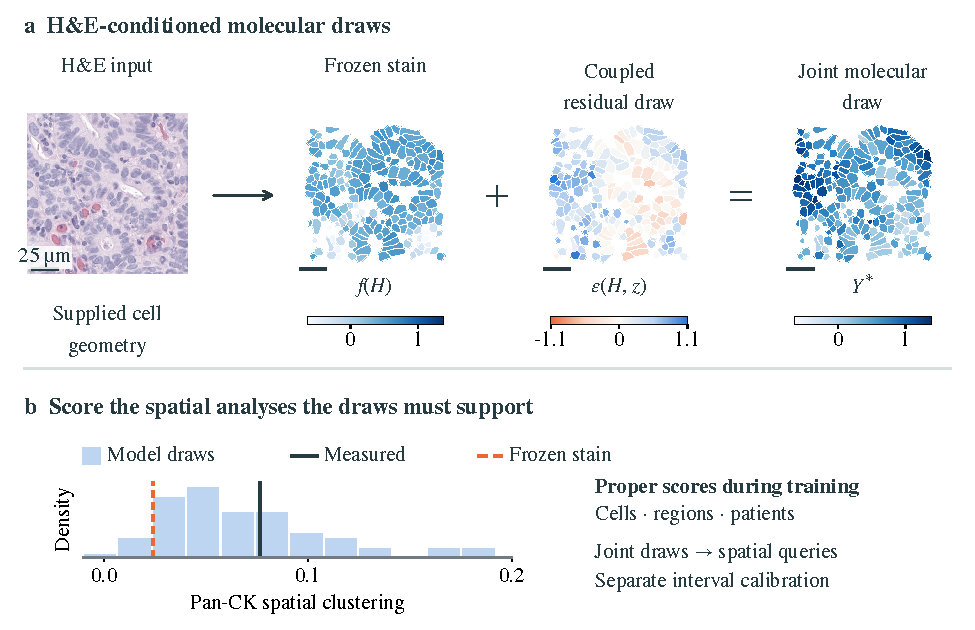
\includegraphics[width=\linewidth]{fig_overview.pdf}
\caption{\method{} generates molecular values jointly in tissue space. \textbf{a}, Original H\&E from the selected crop and molecular maps on its 196 retained, assay-segmented cells. The frozen Pan-CK prediction plus a coupled residual gives a joint draw. Views share physical coordinates and image orientation; bars: 25\,$\mu$m. Molecular maps share a standardized-log-intensity scale; residuals use a signed scale. \textbf{b}, All 64 stored clustering draws, with measured and frozen-stain values marked. Training scores cells, regions and patients; intervals require separate calibration. This selected illustration does not establish aggregate accuracy or coverage. The molecular realization is separate from the histogram draws.}
\label{fig:overview}
\end{figure}

\paragraph{Architecture.} Each cell is represented by a frozen pathology foundation-model embedding of its $20.8\,\mu$m H\&E patch (Phikon-v2 \citep{phikon2}, 1024-d, PCA to 128-d fitted on training patients), four nuclear and cell-shape descriptors, and the virtual-stain prediction $f_i$. Three transformer layers attend across all cells of a $166\,\mu$m region with a learned distance-dependent attention bias (16 radial basis functions per head). The primary ORION and lung stains use this transformer trained with per-cell squared error; each wrapper is compared with its own frozen stain's plug-in.

\paragraph{Three-level objective.} For a batch of 4 patients with 4 regions each and $s=1,\dots,16$ joint samples per region,
\begin{equation}
\mathcal{L}=\underbrace{\overline{\mathrm{CRPS}}\big(\mathcal{N}(f_{ia},\textstyle\sigma_{ia}^2),Y_{ia}\big)}_{\text{cell markers}}
+\lambda_r\underbrace{\overline{\mathrm{CRPS}}\big(\{\theta_j(S(\hat Y^{(s)}_r))\},\theta_j(S(Y_r))\big)}_{\text{region statistics}}
+\lambda_p\underbrace{\overline{\mathrm{CRPS}}\big(\{\theta_j(\bar S^{(s)}_g)\},\theta_j(\bar S_g)\big)}_{\text{patient statistics}},
\end{equation}
where the cell term scores a moment-matched Gaussian surrogate by closed-form CRPS, with $\sigma_{ia}^2$ the model's marginal variance, the other terms use the unbiased 16-sample CRPS over all $J=832$ coordinates and bin contrasts of $S$ (16 means, $3\times136$ binned moments, $3\times136$ contrasts) standardized by their standard deviation across training regions, and $\bar S_g$ averages $S$ over the 4 sampled regions of patient $g$ with samples sharing $\eta_g$. We use bins 0--25, 25--50 and 50--75\,$\mu$m, $\lambda_r=\lambda_p=1$, AdamW (learning rate $10^{-3}$ one-cycle, weight decay $10^{-3}$, dropout 0.1), 15 epochs, and early stopping on validation patients. Hyperparameters were fixed before test evaluation. Only the linear residual is resampled, so an epoch over 24 patients takes about 30\,s on 8 CPU cores.

\paragraph{Held-out variance calibration.} A flexible model fit to 24 patients learns their statistics too sharply. After training we freeze the network and fit seven scalars, one log-scale for each variance component (four fields, cell, region, patient), on the validation patients with the same objective. Every downstream statistic inherits this rescaled spread, though raw intervals remain under-covered.

\paragraph{Inference.} For a new slide we draw 64 joint samples (sample $k$ of every region of a patient shares $\eta_{g,k}$). Applying a query to every sample gives its model-based predictive distribution and mean estimate. Held-out query values calibrate its intervals; empirical sample quantiles alone do not guarantee coverage. For gated queries, validation-fitted quantile thresholds (\method{}-Q) adjust predicted positive fractions, using the same information as a quantile-matched plug-in. The resulting cell labels are marker-based proxies for phenotypes.
Bilinear conditional means can also be integrated analytically (Appendix~\ref{app:impl}); nonlinear queries use samples.

\section{Statistical rationale and identification limits}
\label{sec:theory}

\begin{proposition}[Plug-in bias]\label{prop:bias}
Let $\mu=\E[Y\mid H]$ and $\Sigma_{ia,jb}=\Cov(Y_{ia},Y_{jb}\mid H)$. For any predictor $f(H)$,
\[
\E[Q_{w,ab}(Y)\mid H]-Q_{w,ab}(f)=\big[Q_{w,ab}(\mu)-Q_{w,ab}(f)\big]+\frac{1}{|E_w|}\sum_{i\ne j}w(d_{ij})\,\tfrac12\,(\Sigma_{ia,jb}+\Sigma_{ib,ja}).
\]
\end{proposition}
The proof expands $Y=\mu+(Y-\mu)$. For the per-cell-optimal $f=\mu$ the bias is the distance-weighted conditional cross-cell covariance of the molecular residual, the part of molecular organization the image does not reveal; shrinkage adds an attenuation term. Per-cell marginal calibration alone does not determine the cross-cell covariance term.

\begin{proposition}[Sharp identification from per-cell laws]\label{prop:nonid}
Fix marker $a$, a symmetric weight matrix $W$ with zero diagonal, and per-cell predictive laws $Y_{ia}\mid H\sim\mathcal{N}(\mu_i,\sigma_i^2)$. The set of values of $\E[Q(Y)\mid H]=\E[\sum_{i\ne j}W_{ij}Y_{ia}Y_{ja}\mid H]$ over all joint laws with these per-cell marginals is the interval
\[
Q(\mu)+\big[\,\min_{R\in\mathcal{E}_n}\langle \Omega,R\rangle,\ \max_{R\in\mathcal{E}_n}\langle \Omega,R\rangle\,\big],\qquad \Omega_{ij}=W_{ij}\sigma_i\sigma_j,
\]
where $\mathcal{E}_n=\{R\succeq0,\ R_{ii}=1\}$ is the elliptope. Every value in the interval is attained by a Gaussian joint law.
\end{proposition}
\emph{Proof.} $\E[Q\mid H]=Q(\mu)+\sum_{i\ne j}W_{ij}\sigma_i\sigma_j\,\mathrm{Corr}(Y_i,Y_j\mid H)$. Every correlation matrix lies in $\mathcal{E}_n$, and every $R\in\mathcal{E}_n$ is the correlation matrix of the Gaussian law $\mathcal{N}(\mu,\mathrm{diag}(\sigma)R\,\mathrm{diag}(\sigma))$, which has the prescribed marginals. The image of the convex set $\mathcal{E}_n$ under a linear map is an interval. $\square$

The same argument covers cross-marker statistics with bivariate Gaussian per-cell laws (Appendix), again giving an interval with semidefinite endpoints. The endpoints are max-cut-type semidefinite programs, solved with a dual certificate (Appendix).



\begin{proposition}[Scoring the statistics that will be analyzed]\label{prop:proper}
(i) Every $Q_{w,ab}$ whose weight is constant on each bin is a fixed linear functional of $S$. (ii) Let $\theta_1,\dots,\theta_J$ be linear functionals of $S$ and let $\mathrm{CRPS}$ denote the continuous ranked probability score, which is strictly proper for univariate laws with finite mean \citep{gneiting2007}. The expected score $\sum_j\E\,\mathrm{CRPS}(F_{\theta_j},\theta_j(S))$ is minimized exactly by predictive laws whose marginals along every $\theta_j$ equal the true conditional laws of $\theta_j(S)\mid H$. Hence a population minimizer in a generator class containing the truth reproduces the conditional mean and every quantile of each scored statistic.
\end{proposition}
\begin{proposition}[What statistic-level scores identify]\label{prop:ident}
Let a Gaussian residual model around a frozen $f$ have covariance $\Sigma(H)$, with bin averages $\Gamma_{k,ab}(\Sigma)=|E_k|^{-1}\sum_{d_{ij}\in B_k}\tfrac12(\Sigma_{ia,jb}+\Sigma_{ib,ja})$. (i) If the class contains a law whose scored marginals are the true ones, every minimizer of the score of Proposition~\ref{prop:proper} satisfies $\Gamma_{k,ab}(\hat\Sigma)=\E[G_{k,ab}(Y)\mid H]-G_{k,ab}(f)$ for all $k,a,b$, so every bin-constant bilinear statistic, scored or not, has the correct conditional mean. (ii) The means of all scored statistics are invariant to every perturbation of $\Sigma$ with zero bin averages, which includes all within-cell cross-marker covariances; these determine the conditional law of one marker given another in the same cell, which the scores therefore do not identify through their means.
\end{proposition}
Part (ii) is consistent with the failure of conditioning on anchor markers (Section~\ref{sec:discussion}).

Gaussian likelihood and statistic scores weight covariance errors differently under misspecification (Appendix Proposition~\ref{prop:alloc}). In ORION regions only 9.2\% of cell pairs lie within 25\,$\mu$m, so a likelihood fit can attenuate the nearest-bin covariance as much as the plug-in does. The per-cell score is also strictly proper, but only for the per-cell law; by Proposition~\ref{prop:nonid} its minimizers need not reproduce the law of any $\theta_j(S)$. A multivariate energy score on all of $S$ is strictly proper for the joint law, but it is known to be weakly sensitive to dependence and to individual coordinates in high dimension \citep{pinson2013}; a preliminary generator trained this way left attenuation unchanged (Appendix~\ref{app:impl}). We therefore score each analyzed statistic directly.

Sampling a patient's regions independently understates the variance of their average by the design effect $1+(m-1)\bar\rho$ for average cross-region correlation $\bar\rho$ (Appendix Proposition~\ref{prop:deff}).
A statistic-averaged split-conformal construction (Appendix Proposition~\ref{prop:conf}), a special case of conformal risk control \citep{crc2024}, turns the generator's per-statistic means and spreads into patient-level intervals whose expected coverage fraction over a new patient's statistics is at least $1-\alpha$ when the calibration patients are exchangeable and unseen by the model.

\section{Experiments}
\label{sec:experiments}

\paragraph{Data.} ORION-CRC \citep{orion2023} provides same-section H\&E and 19-channel cyclic immunofluorescence with supplied whole-cell segmentation, distributed as 512$\times$512-pixel regions at 0.325\,$\mu$m/pixel. We use all 3,337 crops in the released VitaminP-derived ORION subset, whose source regions were selected for reliable segmentation; this is not a whole-slide sample. Quality control removes tiny/border cells, unmatched nuclei and duplicate cells in overlapping crops (Appendix). The retained dataset has 333,133 cells in 3,331 regions from 40 patients; 3,323 regions contain both near and far cell pairs. Targets are 16 biological markers (CD31, CD45, CD68, CD4, FOXP3, CD8a, CD45RO, CD20, PD-L1, CD3e, CD163, E-cadherin, PD-1, Ki67, Pan-CK, SMA); Hoechst, autofluorescence and the blank channel are excluded. Intensities are $\log(1+x)$ of the mean whole-cell signal, standardized with training-patient statistics only.

\paragraph{Protocol.} Five rotations assign 24 training, 8 validation and 8 test patients so that every patient is a test patient exactly once. Validation patients are used for early stopping, for \method{}'s variance calibration and to fit the calibration baselines; no test-patient protein enters any fitted quantity. Contrast evaluation uses regions with both near and far pairs. We evaluate all 136 marker pairs (120 cross-marker, 16 same-marker) with the near (0--25\,$\mu$m) minus far (50--75\,$\mu$m) contrast at the patient level. Pooled summaries use each fold's training-standardized coordinates, rather than common assay units. Errors are normalized per statistic by the plug-in's patient-level mean squared error (MSE) and then averaged. Relative bias is the cohort-mean error divided by the measured mean, summarized over statistics with $|$measured mean$|>0.02$. Reported $p$-values are exploratory and unadjusted for multiplicity; patient-bootstrap intervals quantify sampling uncertainty conditional on the fitted models, not model-selection uncertainty.

The reference run, reseed mean, four-run aggregate and rerotation are distinguished in Appendix Table~\ref{tab:runregistry}; independent calibration uses separate patient roles.

\paragraph{Baselines.} The plug-in uses the frozen stain's per-cell predictions (test cell MSE 0.78). Global rescaling fits one slope shared across statistics on validation regions. The matched direct graph receives the same embeddings and stain predictions, uses the same transformer, and predicts Gaussian laws for the scored statistic vector with region- and patient-level CRPS. It predicts statistics rather than cell measurements.

Additional controls are per-statistic affine calibration on validation regions; direct ridge regression without stain inputs, from region feature means/standard deviations, cell count and binned products of the leading 16 components, with its penalty chosen on validation patients; and independent region draws from \method{}, removing cross-region dependence. Three simple baselines were added post hoc, after test results were seen (Appendix~\ref{app:simple}). Ablations are in Section~\ref{sec:ablations}.
\section{Results}
\label{sec:results}



\subsection{Spatial-statistic estimation on held-out patients}
\begin{table}[t]
\centering
\caption{Patient-level estimation of 136 spatial statistics over 40 held-out patients (24/8/8 training/validation/test rotations). MSE is relative to the plug-in (lower is better); bias is the median relative cohort-mean error; $\rho$ is Spearman correlation with measured values across patients; CRPS treats point estimates as point masses. $^\dagger$Post hoc; one validation-fitted shift per statistic.}
\label{tab:main}
\begin{tabular}{@{}lccccccc@{}}
\toprule
& \multicolumn{3}{c}{MSE / plug-in} & \multicolumn{2}{c}{bias} & & \\
\cmidrule(lr){2-4}\cmidrule(lr){5-6}
Method & all & cross & same & all & same & $\rho$ & CRPS \\
\midrule
Plug-in & 1.00 & 1.00 & 1.00 & $-34\%$ & $-58\%$ & 0.52 & 0.040 \\
Per-statistic calibration & 1.13 & 1.17 & 0.78 & $0\%$ & $0\%$ & 0.41 & 0.042 \\
Plug-in + constant$^\dagger$ & \BaseRefConstAll{} & \BaseRefConstCross{} & \BaseRefConstSame{} & $\BaseRefConstBiasAll\%$ & $\BaseRefConstBiasSame\%$ & \BaseRefConstRho{} & -- \\
Direct ridge regression & 1.42 & 1.48 & 0.99 & -- & -- & 0.31 & -- \\
Direct graph (stain inputs) & 0.89 & 0.93 & 0.63 & -- & -- & 0.53 & -- \\
Global rescale of plug-in & 0.89 & 0.90 & 0.83 & $-18\%$ & $-49\%$ & 0.54 & -- \\
Calibrated Gaussian plug-in & 1.00 & 1.00 & 1.00 & $-34\%$ & $-58\%$ & 0.52 & \GaussianCRPS{} \\
\method{} (reference run) & 0.88 & 0.92 & 0.60 & $-6\%$ & $-5\%$ & 0.53 & \RefCRPS{} \\
\method{} (four-run aggregate) & \SeedAllMSE{} & \SeedCrossMSE{} & \SeedSameMSE{} & $-6\%$ & $-4\%$ & 0.52 & \AggregateCRPS{} \\
\bottomrule
\end{tabular}\\[3pt]
Except for the four-run aggregate, rows use the reference evaluation. Gaussian plug-in: per-statistic validation variance (90\% coverage 86\%, width 0.19). Reference \method{} coverage: \RefCoverage\% raw, 90.9\% after validation inflation (width 0.18); independently sampled regions: \IndependentCoverage\%. The four-run aggregate row averages per-run metrics, not predictions; the reference run has the lowest overall MSE of those four.
\end{table}

The four-run aggregate of \method{} has relative MSE \SeedAllMSE{} overall and \SeedSameMSE{} for clustering; the direct graph (stain inputs), reseed mean, has \DirectAllMSE{} and \DirectSameMSE{} (Appendix Table~\ref{tab:primaryseeds}). The direct model has lower overall error; the clustering difference is not statistically significant. The evidence favoring \method{} over direct prediction concerns calibrated overall forecasts; reusing samples avoids a new fit, without an established accuracy or cost advantage.

The reference run reduces median cohort attenuation from 34\% to 6\% overall and 58\% to 5\% for clustering (Appendix Fig.~\ref{fig:main}a). Relative MSE is \RefMSE{} overall (patient-bootstrap 95\% interval 0.833--1.002) and 0.60 for clustering (0.54--0.73). Clustering error is lower in 36 of 40 patients ($p=5\times10^{-7}$); the overall per-patient improvement is not statistically significant ($p=0.09$, 24 of 40 patients). Global rescaling is competitive overall (0.89) and slightly better on cross-marker statistics (0.90 vs 0.92), but leaves $-18\%$ median bias and higher clustering MSE (0.83 vs 0.60). One validation-fitted constant per statistic removes more of the cohort bias (median $\BaseRefConstBiasAll\%$), with MSE \BaseRefConstAll{} overall and \BaseRefConstSame{} for clustering, so bias correction accounts for most of the clustering gain; \method{}'s MSE difference from it is $\BaseRefDiffAll$ overall ($[\BaseRefDiffAllLo,\BaseRefDiffAllHi]$) and a borderline $\BaseRefDiffSame$ for clustering ($[\BaseRefDiffSameLo,\BaseRefDiffSameHi]$), with better patient ranking (\BaseRefLigRho{} vs \BaseRefConstRho{}).

Reference-run CRPS is \RefCRPS{} versus \GaussianCRPS{} for a calibrated Gaussian plug-in: \CRPSReduction\% lower. It is lower than the point-mass plug-in's 0.040 in all 40 patients ($p=2\times10^{-12}$). Mean patient-ranking correlation changes little overall (0.52 to 0.53), with a larger change for clustering (0.55 to 0.60); cohort bias correction and patient discrimination are distinct outcomes.



\subsection{Patient-level uncertainty}
Independent calibration separates selection from calibration: stain and generator are retrained on 20 patients per rotation, 2 serve selection/variance fitting, and 10 serve calibration only. We extend this protocol to three fixed residual/direct-model seeds, reusing the five stains. All 40 patients are tested once per seed; metrics are averaged across seeds, not ensembles. Each method receives the same per-statistic split-conformal calibration. Adaptive intervals scale with predicted spread; constant-scale controls use the same predicted center (Fig.~\ref{fig:benchmark}; Table~\ref{tab:forecast}).

Across all 136 statistics, \method{}'s adaptive interval score is 10.6\% below the matched direct graph's (difference $-0.59$, paired patient-bootstrap 95\% interval $[-0.87,-0.31]$), with coverage 90.5\% versus 90.9\%. Widths are nearly equal (3.72 versus 3.75); the difference comes from smaller miss penalties (1.26 versus 1.82). Its score is also 12.2\% below its own constant-scale control (difference $-0.69$, interval $[-0.98,-0.41]$), indicating information in the spread beyond the center. These overall comparisons are exploratory and largely driven by cross-marker forecasts. The prespecified clustering score difference from the direct graph is not statistically significant ($-0.50$, interval $[-1.11,0.11]$), and the width-difference interval also includes zero. Point-MSE ratios are 0.95 for \method{} and 0.96 for direct prediction; the difference is not statistically significant. Raw sample quantiles cover only 70.2\% overall and 44.8\% for clustering. These development-cohort checks are not independent confirmation (Appendix~\ref{app:querybench}).

Post hoc baselines do not close the overall gap but are not separated on clustering (Table~\ref{tab:forecast}; Appendix~\ref{app:simple}). \method{}'s difference from the plug-in plus one constant is $\BaseLigConstScore$ ($[\BaseLigConstScoreLo,\BaseLigConstScoreHi]$; clustering $\BaseLigConstSameScore$, $[\BaseLigConstSameScoreLo,\BaseLigConstSameScoreHi]$), a baseline the direct graph only ties ($\BaseDirConstScore$, $[\BaseDirConstScoreLo,\BaseDirConstScoreHi]$); a variant using in-sample plug-ins has lower point error (MSE \BaseInsampleAll{}, clustering \BaseInsampleSame{}) at score \BaseInsampleScore{}. The difference from a stain-context ridge is $\BaseLigRidgeScore$ ($[\BaseLigRidgeScoreLo,\BaseLigRidgeScoreHi]$). That ridge's penalty selection on two patients is erratic: fixed penalties from 10 to $10^4$ reach MSE \BaseFixedAllLo--\BaseFixedAllHi{} (clustering \BaseFixedSameLo--\BaseFixedSameHi), at or below \method{}'s 0.95 (0.66), with no penalty scoring below \BaseFixedMinScore{} overall.

\begin{figure}[t]
\centering
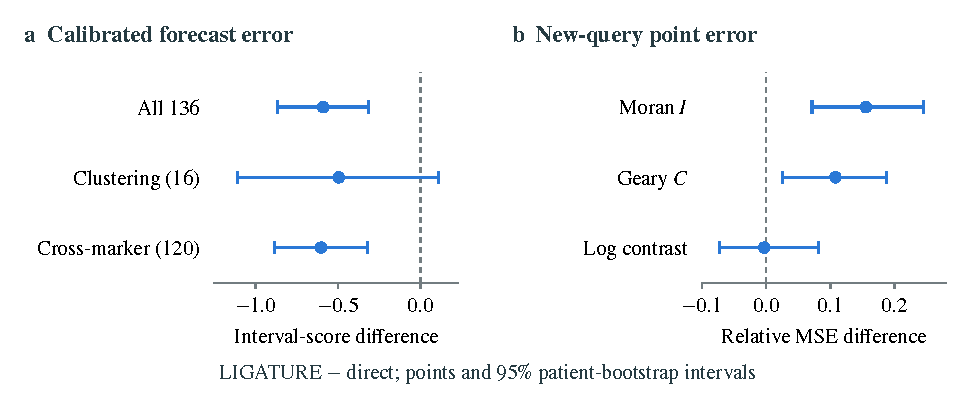
\includegraphics[width=\linewidth]{fig_benchmarks.pdf}
\caption{Complete three-seed comparison under independent calibration, all 40 patients. Differences are \method{} minus the matched direct graph: negative favors \method{}. \textbf{a}, Training-standard-deviation-normalized 90\% interval score; overall coverage is 90.5\% versus 90.9\%. \textbf{b}, Plug-in-normalized point MSE for queries excluded from generative training; the direct head is trained on these queries. Points average seed metrics; bars are conditional 95\% patient-bootstrap intervals. The overall forecast comparison is exploratory; clustering includes zero, while the new autocorrelation queries favor direct prediction.}
\label{fig:benchmark}
\end{figure}

\begin{table}[t]
\centering
\caption{Independent calibration (20/2/10/8 roles), three seeds and 40 test patients. Direct denotes the graph with stain inputs. MSE is relative to the protocol's plug-in. Coverage, width and 90\% interval score summarize all 136 statistics; width and score use training-patient standard deviations (lower is better). All intervals use the same ten calibration patients per rotation. $^\dagger$Post hoc (Appendix~\ref{app:simple}).}
\label{tab:forecast}

\begin{tabular}{@{}lrrrrr@{}}
\toprule
& \multicolumn{2}{c}{MSE / plug-in} & & & \\
Method / interval & all & same & Coverage & Width & Score \\
\midrule
Plug-in / constant & 1.00 & 1.00 & 91.5\% & 4.09 & 5.89 \\
Global rescale / constant & 1.85 & 1.07 & 90.6\% & 4.88 & 7.13 \\
No-image mean$^\dagger$ / constant & 1.63 & 1.34 & 89.8\% & 4.62 & 6.78 \\
Plug-in + constant$^\dagger$ / constant & 1.01 & 0.73 & 90.9\% & 3.89 & 5.58 \\
Stain-context ridge$^\dagger$ / constant & 1.03 & 0.71 & 90.9\% & 4.01 & 5.80 \\
Direct / adaptive & 0.96 & 0.75 & 90.9\% & 3.75 & 5.57 \\
\method{} / adaptive & 0.95 & 0.66 & 90.5\% & 3.72 & 4.98 \\
\method{} / constant & 0.95 & 0.66 & 91.1\% & 3.99 & 5.67 \\
\bottomrule
\end{tabular}

\end{table}

The reference pipeline is exploratory because its validation patients also serve selection and variance fitting. Raw 90\% intervals cover \RefCoverage\% overall (Appendix Fig.~\ref{fig:main}c), versus \IndependentCoverage\% with independently sampled regions. Validation inflation yields 90.9\% (86--96\% across rotations), but clustering coverage remains 50\% raw and 76\% inflated. Statistic-averaged conformal intervals with $\alpha=0.15$ cover 97\% overall and 91\% for clustering; validation reuse prevents an exact finite-sample guarantee for this protocol. Its plug-in control also covers (92\%), with clustering intervals 1.8 times wider.

Calibrating held-out values of unscored queries gives conformal 90\% intervals for gated contact fractions and neighborhood frequencies that cover 91.6\% and 92.8\% (raw: 46\% and 44\%). They are about as wide as identically calibrated quantile-matched plug-in intervals, with 26\% and 24\% lower patient-averaged squared error (Table~\ref{tab:unscoredcal}); 25\% of adaptive contact intervals span all of $[0,1]$.

\subsection{Six virtual stains, including two published models}
We wrapped five further stains without changing \method{} (Appendix Table~\ref{tab:stains}): a per-cell ridge regression on the same embeddings (no spatial context); a pixel-level U-Net trained on H\&E at 0.65\,$\mu$m/pixel with pixel and per-cell losses, the architecture class of published image-to-image stains; two published models run on ORION H\&E without fine-tuning; and one of them, GigaTIME, fine-tuned end to end on training patients. ROSIE \citep{rosie2025} covers all 16 of our markers and GigaTIME \citep{gigatime2025} 9; both are mapped to ORION intensities on training patients (Appendix~\ref{app:impl}).

Attenuation depends strongly on the stain: $-68\%$ and $-94\%$ for GigaTIME and ROSIE under the domain shift from their training platforms, $-34$ to $-39\%$ for the cell-level stains, and $-12\%$ and $-7\%$ for the U-Net and fine-tuned GigaTIME. \method{} brings the median bias to within 8\% for every stain. Relative to each stain's own plug-in, point-estimate gains track the attenuation: patient-level MSE is 0.61 and 0.73 for ROSIE and GigaTIME, 0.86--0.88 for the cell-level stains, and 1.04 for the U-Net and 0.96 for fine-tuned GigaTIME. Probabilistic accuracy improves for every stain (CRPS 10--34\% below a calibrated Gaussian plug-in), and for gated contact fractions \method{} has lower error than the quantile-matched plug-in for every stain (0.40--0.72 vs 0.63--1.71 of the plug-in's).

\paragraph{A common scale.} Dividing every estimator's per-statistic MSE by the transformer plug-in's (Table~\ref{tab:common}) shows what \method{} takes from a stain. In the reference run, predicting the trained statistics directly is competitive: a graph model with the same embeddings, transformer and CRPS scores has 1.30 times the plug-in's error without the stain, and 0.89 (0.63 for clustering) with the stain's predictions as inputs, against 0.88 (0.60) for \method{} (lung: 0.82 vs 0.84; CRPS within 5\% either way). Scoring the statistics matters too: the same backbone fitted by a regularized conditional Gaussian likelihood has 2.7 times the plug-in's error, worse than the attenuation Proposition~\ref{prop:alloc} describes. \method{} around a constant stain reaches 1.13 (1.00 with a learned mean; 0.76 and 0.75 for clustering), and the published stains applied across platforms add nothing to it (wrapped ROSIE 1.17, GigaTIME 1.14), so their gains over their own plug-ins measure how much \method{} repairs a poorly transferred stain.

\paragraph{Why pixel-level stains look unbiased.} They omit as much residual second moment as the other in-domain stains, but a negative predictor--residual cross term, which vanishes for a conditional mean, offsets it in the cohort mean (Appendix Table~\ref{tab:biasdec}); a frozen-mean wrapper cannot undo it.



\subsection{A separate cohort, platform and modality}
We applied the identical pipeline, with no hyperparameter changed, to the 20 lung Xenium samples of HEST-1k \citep{hest2024}, from 19 patients of a pulmonary fibrosis study \citep{vannan2025} (15 fibrotic, 5 control samples): same-section H\&E with in situ transcript counts, so tissue, disease, platform, molecular modality and segmentation all differ from ORION. We built 1{,}600 regions of 166\,$\mu$m (216{,}102 cells) and took 16 genes spanning epithelial, immune, stromal and endothelial lineages (Appendix), with library-normalized counts as targets and patient rotations as before (11 training, 4 validation, 4 test). Results are in Table~\ref{tab:lung}.

The plug-in attenuates the statistics by a median of 71\%. \method{} lowers patient-level MSE to 0.84 of the plug-in's overall ($p=0.005$; 13 of 19 patients) and 0.48 for clustering ($p=3\times10^{-5}$; 17 of 19), and its CRPS is 23\% below the calibrated Gaussian plug-in's in all 19 patients ($p=4\times10^{-6}$). A global rescale gains nothing (1.03), the direct graph model reaches 0.93 (0.82 with the stain as input) and \method{} around a constant stain 0.90--0.91, so here the stain adds to the encoder. For gated contact fractions \method{}-Q's error is 46\% below the quantile-matched plug-in's, again in all 19 patients ($p=4\times10^{-6}$).

Attenuation is only partly removed (median bias $-23\%$; one validation-fitted constant per statistic gives $\BaseLungConstBiasAll\%$, with MSE \BaseLungConstAll{} overall and \BaseLungConstSame{} for clustering), and raw 90\% intervals cover 64\% (89\% after inflation); a patient-disjoint refit with 4 calibration patients, enough only for an 80\% target, covers 82.6\% of clustering statistics with intervals 19.5\% narrower than the calibrated plug-in's, though a constant-scale interval around \method{}'s mean is narrower still at a similar score (Table~\ref{tab:lungcal}).

\begin{table}[t]
\centering
\caption{Separate lung cohort (Xenium, 19 held-out patients): patient-level MSE relative to the plug-in over 136 gene-pair statistics (all) and the 16 clustering statistics (same), mean Spearman correlation with measured values, and median relative bias of cohort means.}
\label{tab:lung}
\begin{tabular}{@{}lcccc@{}}
\toprule
Estimator & MSE all & MSE same & $\rho$ & bias \\
\midrule
Plug-in (cell-graph transformer stain) & 1.00 & 1.00 & 0.46 & $-71\%$ \\
Global rescale of the plug-in & 1.03 & 0.83 & 0.45 & $-60\%$ \\
Direct graph model (statistics, no cells) & 0.93 & 0.55 & 0.39 & $-21\%$ \\
\method{} around a constant stain & 0.91 & 0.52 & 0.43 & $-18\%$ \\
\method{} around a constant stain, learned mean & 0.90 & 0.53 & 0.47 & $-24\%$ \\
Direct graph with stain inputs (statistics, no cells) & 0.82 & 0.49 & 0.49 & $-24\%$ \\
\method{} around the transformer stain & 0.84 & 0.48 & 0.48 & $-23\%$ \\
\bottomrule
\end{tabular}

\end{table}

\subsection{Statistics never scored in training}
\label{sec:unscored}
Because \method{} produces joint samples, nonlinear statistics are computed on samples exactly as on measured data. The most widely used are gated contact statistics, such as the fraction of CD8+ T cells adjacent to tumor cells; we use marker gates as a proxy for such phenotypes. We marked a cell positive for a marker when its value exceeds the training-patient 85th percentile and computed, for all 256 ordered marker pairs, the fraction of $a$-positive cells with a $b$-positive cell within 20\,$\mu$m, pooling counts over each patient's regions (patients with at least 20 measured $a$-positive cells). This statistic is a neighborhood maximum, not a product moment, and was never part of any loss. The plug-in thresholded at the same cut-off underestimates it (median bias $-26\%$); a quantile-matched plug-in, thresholded at its own 85th percentile on validation patients so that positive fractions match, removes most of the bias ($-6\%$) and lowers error to 0.88 times the plug-in's. \method{} lowers it to 0.62 (median 0.55; bias $+9\%$), with lower error than the quantile-matched plug-in for 83\% of pairs and in 29 of 40 patients (paired Wilcoxon $p=9\times10^{-5}$; MSE ratio 0.70, patient-bootstrap 90\% interval 0.65--0.83), and raises the mean rank correlation from 0.50 to 0.59. Per-pair results are in Table~\ref{tab:contactex}. Raw 90\% interval coverage for these statistics is 52\%.

With quantile-matched thresholds (\method{}-Q), contact error falls to 0.56 and is below the quantile-matched plug-in's for 97\% of pairs. A direct graph model trained on the contact fractions themselves (three seeds; Appendix~\ref{app:impl}) ties \method{}-Q (0.59 vs 0.56; lung 0.15 vs 0.17; paired 95\% intervals $-0.07$ to 0.06 and 0.00 to 0.05): \method{} matches it without training on contacts, but only with matched thresholds.

The same holds for per-patient cellular neighborhood frequencies \citep{schurch2020} (eight gated types; 10 neighborhoods of 10-nearest-neighbor compositions, fitted on training patients). Unmatched \method{} does not beat the quantile-matched plug-in (total-variation distance to the measured profile 0.36 vs 0.34), because its Gaussian residual over-calls positive cells; \method{}-Q does (0.29, Wilcoxon $p=0.005$; per-neighborhood MSE 0.53 vs 1.17 of the plug-in's, clusters aligned across rotations), and does so for every stain in Appendix Table~\ref{tab:stains} (0.28--0.36 vs 0.33--0.54, $p\le0.006$ each; Table~\ref{tab:cn}), including the U-Net. A Gaussian copula (training on per-marker normal scores) removes the need for matched thresholds (unmatched: neighborhood distance 0.30, $p=5\times10^{-4}$; contact error 0.59). Other gates and three further query families behave similarly (Appendix~\ref{app:families}).

\paragraph{Limits of query reuse.} In the three-seed independent protocol, frozen samples improve Moran's $I$ and Geary's $C$ over the plug-in (MSE ratios 0.43 and 0.46), but an adapted direct graph is better (0.27 and 0.35; paired Holm-adjusted $p=0.003$ and $0.009$), as is a cheap frozen-feature ridge (0.21 and 0.29). Post hoc, a no-image training mean reaches \BaseMoranNoImage{} and \BaseGearyNoImage{} and the plug-in plus one constant \BaseMoranConst{} and \BaseGearyConst{}, and both have better interval scores than \method{}'s adaptive intervals (Moran \BaseMoranNoImageScore{} and \BaseMoranConstScore{} vs 7.89; Geary \BaseGearyNoImageScore{} and \BaseGearyConstScore{} vs 6.32), so the gain over the plug-in does not show added image information. Preserving the exact within-cell marginal law while removing cross-cell dependence gives 2.24 and 3.16: samples fail on these ratios without cross-cell dependence, but dependence does not make them accurate. Inverting fold standardization before clustering evaluation gives much smaller improvements on the original log-assay scale (sample mean 0.98, analytic mean 0.96 of the plug-in's MSE). The larger standardized-contrast gains are estimand dependent.



\paragraph{Downstream checks.} Neither association-study error (0.099 vs 0.149 for the plug-in; 90\% interval for the reduction $-2\%$ to 40\%) nor predictive-spread triage (50\% of error removed by measuring 20\% of patients, vs 51\% by plug-in magnitude) establishes additional biological utility (Appendix Fig.~\ref{fig:downstream}b,c).

\subsection{Ablations}
\label{sec:ablations}


Across 36 ablation variants, statistic-level scores, bin contrasts, morphology-dependent loadings and shared patient variation matter most (Appendix Tables~\ref{tab:ablation},\ref{tab:ablationfull}). Removing spatial fields raises overall MSE to \CurrentNoFieldsMSE{} (lung 0.94 vs 0.84--0.86) but leaves ORION clustering (0.62) and CRPS (0.0282) within seed variation; one field scale or rank 1 also stays within noise. The reseed mean has MSE $\SeedMSEMean\pm\SeedMSESD$, with raw coverage $\SeedCoverageMean\pm\SeedCoverageSD\%$. In the rerotation, with the stain retrained, \method{} has MSE 0.93 overall and 0.64 for clustering, with median bias reduced from $-34\%$ to $-5\%$; the direct graph (stain inputs) has 0.91 and 0.69. Cell-only training gives MSE \CurrentCellOnlyMSE{}; removing the patient latent gives raw coverage \CurrentNoPatientCoverage\%. Earlier-run variants are labeled separately. Independent Gaussian per-cell residuals with fitted marginal variances leave attenuation unchanged and cover 28\%, consistent with Proposition~\ref{prop:nonid}.

\subsection{Dependence targeted by the generator}
For model-implied Gaussian per-cell marginals, the certified identification interval for expected clustering is a median 2.4 times the statistic's 5--95\% cohort range: per-cell laws leave this much dependence unspecified (Appendix~\ref{app:diagnostics}).

\paragraph{Known-law simulations.} We simulate residuals from the model class on ORION geometry with the frozen stain as the true conditional mean (Table~\ref{tab:sim}). The Bayes per-cell plug-in still attenuates contrasts by 38\% (clustering 61\%). \method{} removes attenuation (median bias $+1\%$), with MSE ratios 0.59 overall and 0.12 for clustering, versus 0.32 and 0.07 for the oracle statistic predictor. Near-bin cross-marker residual correlations agree with truth ($r=0.97$). Added within-cell factors with correlations 0.22 and 0.36 remain unrecovered (0.01 and $-0.20$) with contrast MSE 0.61 overall and 0.12 for clustering, consistent with Proposition~\ref{prop:ident}(ii).

\paragraph{Non-touching-pair sensitivity.} A fixed-model check excludes near pairs whose supplied masks are within two pixels in Chebyshev distance (0.65\,$\mu$m per axis), removing \ControlRemovedPercent\% of near pairs. On \ControlRegions{} retained regions and all 40 patients, clustering MSE is \ControlMSE{} of the matched plug-in's (95\% patient-bootstrap interval \ControlLower--\ControlUpper); median signed bias changes from $\ControlPluginBias\%$ to $\ControlJointBias\%$. The error reduction is not statistically significant. This narrow mask-distance sensitivity does not resolve optical spillover or segmentation artifacts (Appendix Table~\ref{tab:segmentation}).

\paragraph{H\&E-derived geometry.} A single-seed control segments H\&E nuclei with InstanSeg \citep{instanseg2024}, adds 1.95\,$\mu$m rims, re-extracts features and refits all models. Across 40 patients and 79,600 cell proxies, clustering MSE is 0.70 of its own plug-in's (95\% interval 0.62--0.89), versus 0.72 for the direct graph. Overall calibrated interval score is 12.2\% below the direct model's at 90.6\% coverage for both. These proxy targets differ from the primary whole-cell targets; optical artifacts remain unresolved (Appendix Table~\ref{tab:hegeometry}).

\section{Discussion}
\label{sec:discussion}

\method{} trains a shared molecular representation against spatial analyses: the same joint draws support scored statistics and additional queries without refitting the generator. Compared with the matched direct graph, its supported advantage is a lower calibrated overall interval score, an exploratory ORION result driven by cross-marker forecasts that also holds against simple post hoc baselines; a point-prediction advantage is not demonstrated. One constant per statistic removes cohort bias and much of the clustering gain, so attenuation alone does not justify a generator. For a fixed query, direct prediction can be cheaper and more accurate, as on the new Moran and Geary queries. Ablations and independent-cell controls support statistic-level scoring, cross-cell dependence and shared patient variation; the identification analysis characterizes dependence left unspecified by the scores.

\paragraph{Limitations.} Validation concerns selected statistics, not the full molecular joint law; samples are model realizations. Both cohorts (40 and 19 patients) were examined during development, and lung models are refitted within cohort. The mask-exclusion check does not correct spillover, so some measured clustering may reflect assay artifacts. Statistics use observed crop pairs without edge correction.

Percentile gates are phenotype proxies, and Gaussian residuals misfit marker tails; a copula helps gated queries. Calibration needs labeled patients. Clustering gains depend on intensity scale, and cross-platform stains understate their in-domain accuracy. All six stains are deterministic; we did not benchmark diffusion or adversarial translators that sample images directly. Anchor-marker conditioning failed (Table~\ref{tab:hybrid}), consistent with Proposition~\ref{prop:ident}(ii).

\paragraph{Code availability.} \url{https://github.com/ark248/LIGATURE}; core release: \path{release/ligature}.

\clearpage
\bibliographystyle{unsrtnat}
\bibliography{refs}

\clearpage
\appendix
\section*{Appendix}
\setlength{\tabcolsep}{3pt}
\begin{figure}[!htp]
\centering
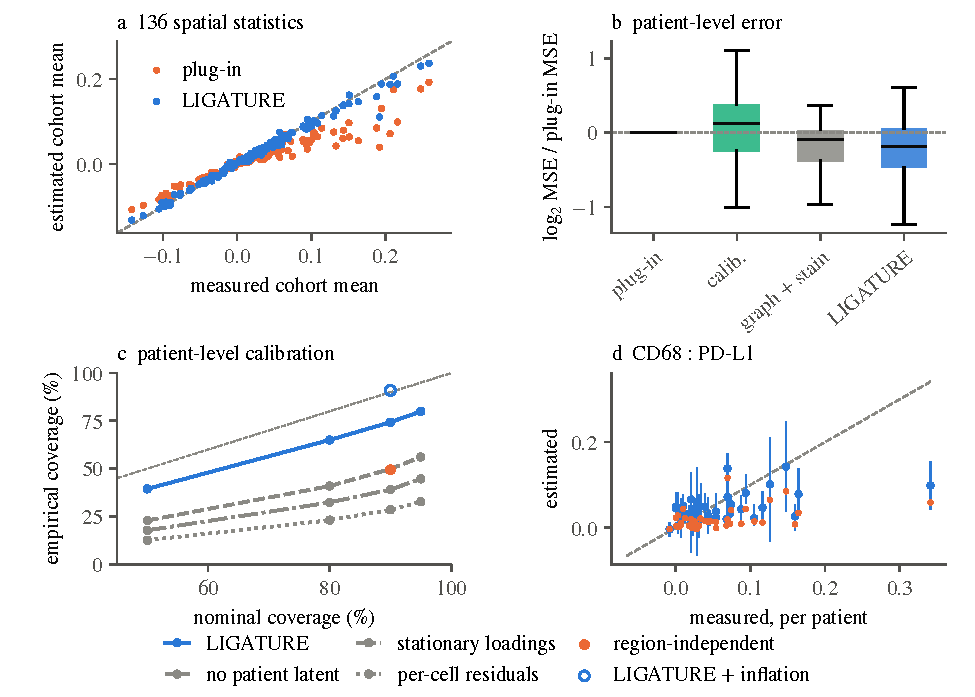
\includegraphics[width=\linewidth]{fig_main.pdf}
\caption{\textbf{a}, Cohort-mean estimate against measured value for the 136 statistics. \textbf{b}, Reference-run patient-level MSE relative to the plug-in, per statistic (boxes: quartiles; whiskers: 1.5 IQR). The direct graph uses stain inputs and is the matched Table~\ref{tab:main} comparator; the weaker direct ridge is omitted. \textbf{c}, Empirical against nominal coverage of patient-level intervals, averaged over statistics, for \method{}, its ablations without patient latent or with stationary loadings, and calibrated per-cell residuals sampled independently. \textbf{d}, CD68--PD-L1 co-localization with reference-run raw 90\% intervals; the high-measured-value patient is missed, illustrating undercoverage.}
\label{fig:main}
\end{figure}
\begin{figure}[!htp]
\centering
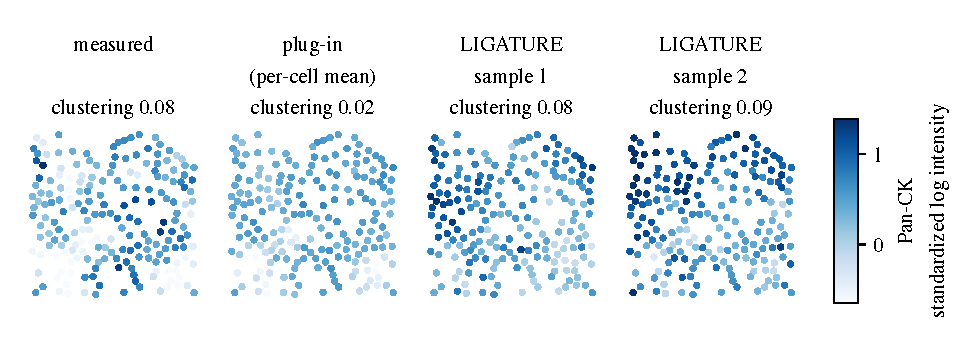
\includegraphics[width=\linewidth]{fig_maps.pdf}
\caption{An illustrative held-out region (patient CRC01, 196 cells), selected automatically as the largest of the 15 test regions whose measured Pan-CK clustering is closest to the fold median. The measured near-minus-far contrast is 0.08, the plug-in gives 0.02, and two model draws give 0.08 and 0.09. These draws illustrate the representation used for statistical inference, with the frozen stain as their mean.}
\label{fig:maps}
\end{figure}
\begin{figure}[!htp]
\centering
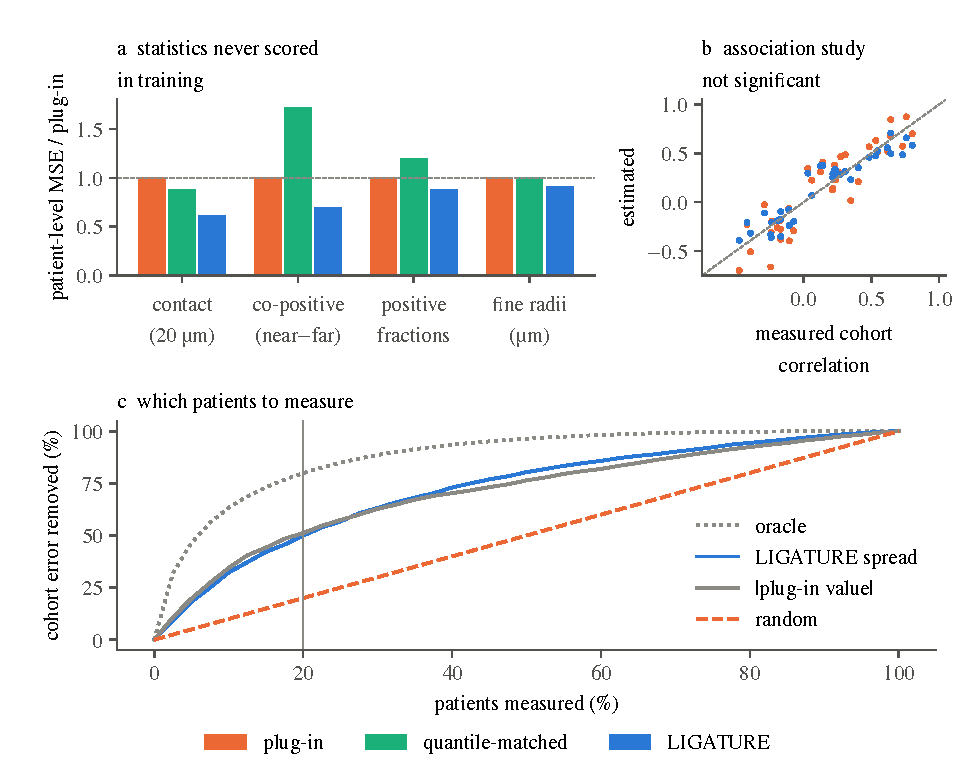
\includegraphics[width=\linewidth]{fig_downstream.pdf}
\caption{\textbf{a}, Patient-level MSE for statistic families never scored in training: gated contact fractions within 20\,$\mu$m (256 ordered pairs), near-minus-far co-positivity, positive-cell fractions, and products at 0--12.5 versus 12.5--25\,$\mu$m. \textbf{b}, Spearman correlation across 40 patients between pairs of nine predefined spatial biomarkers. The reduction in correlation-estimation error is not statistically significant (90\% bootstrap interval includes zero). \textbf{c}, Fraction of cohort squared error removed by measuring patients in order of \method{}'s predictive spread, of the magnitude of the plug-in value (a mean-only control), at random, or by an oracle, averaged over the 136 statistics.}
\label{fig:downstream}
\end{figure}

\paragraph{Identification computations.} The endpoints are max-cut-type semidefinite programs, which we solve by Riemannian ascent on $R=VV^\top$ \citep{boumal2016} (unit rows, rank $k>\sqrt{2n}$), certify with the dual bound $\sum_iy_i+n\max(0,-\lambda_{\min}(\mathrm{diag}(y)-\Omega))$, $y_i=(\Omega VV^\top)_{ii}$, and round into explicit rank-one Gaussian witnesses $Y_i=\mu_i+\sigma_is_iZ$, $s=\mathrm{sign}(Vg)$ \citep{goemans1995}. A procedure that specifies only per-cell predictive laws (heteroscedastic heads, per-cell conformal intervals, ensembles or multiple imputation sampled independently per cell) determines a spatial statistic only up to this interval; we compute it on real tissue in Section~\ref{sec:results}. Hyperplane rounding gives explicit rank-one Gaussian couplings with the prescribed per-cell laws that reach a median 90\% (minimum 80\%) of the upper endpoint, and the dual bound is within 0.33\% of every computed upper endpoint and 4.9\% (median 0.26\%) of every lower endpoint; certified outer bounds widen patient-level intervals by at most 0.29\%. The restricted interval uses stationary, nonnegative correlations decaying with distance: mixtures of exponential kernels with ranges 5--160\,$\mu$m plus a nugget, for which the endpoints are closed form.

\paragraph{Patient-level uncertainty.}
\begin{proposition}[Patient-level uncertainty]\label{prop:deff}
For a patient with region statistics $Q_1,\dots,Q_m$, $\Var(\bar Q\mid H)=m^{-2}\sum_c\Var(Q_c\mid H)+m^{-2}\sum_{c\ne c'}\Cov(Q_c,Q_{c'}\mid H)$. A generator that samples regions independently sets the second term to zero and, with equal region variances, understates the variance by the design effect $1+(m-1)\bar\rho$ for average cross-region correlation $\bar\rho$.
\end{proposition}

\paragraph{Statistic-averaged split conformal.}
\begin{proposition}[Statistic-averaged split conformal]\label{prop:conf}
Let patients $1,\dots,n+1$ be exchangeable, with normalized scores $r_{iq}=|Q_{iq}-\hat\mu_{iq}|/\hat s_{iq}$ for statistics $q=1,\dots,J$, where $\hat\mu,\hat s$ are the generator's sample mean and standard deviation, computed by a model that did not see these patients. Let $g_i(t)=J^{-1}\sum_q\mathbf{1}\{r_{iq}\le t\}$ and $\hat\tau=\inf\{t:(n+1)^{-1}\sum_{i\le n}g_i(t)\ge1-\alpha\}$. Then the intervals $\hat\mu_{n+1,q}\pm\hat\tau\hat s_{n+1,q}$ satisfy $\E[g_{n+1}(\hat\tau)]\ge1-\alpha$: the expected fraction of a new patient's statistics that are covered is at least $1-\alpha$.
\end{proposition}
\emph{Proof.} Let $A(t)=(n+1)^{-1}\sum_{i\le n+1}g_i(t)$ and $\tau^*=\inf\{t:A(t)\ge1-\alpha\}$, a symmetric function of the $n+1$ patients. Since $g_{n+1}\ge0$, $(n+1)^{-1}\sum_{i\le n}g_i(t)\le A(t)$ for all $t$, so $\{t:(n+1)^{-1}\sum_{i\le n}g_i(t)\ge1-\alpha\}\subseteq\{t:A(t)\ge1-\alpha\}$ and $\hat\tau\ge\tau^*$; as $g_{n+1}$ is nondecreasing, $\E[g_{n+1}(\hat\tau)]\ge\E[g_{n+1}(\tau^*)]=\E[(n+1)^{-1}\sum_{i\le n+1}g_i(\tau^*)]\ge1-\alpha$ by exchangeability. $\square$ This is conformal risk control \citep{crc2024} with the miscovered-fraction loss, bounded by one. The guarantee holds for dependent statistics within a patient and needs $1-\alpha\le n/(n+1)$; with $n=8$ validation patients we use $\alpha=0.15$.

\begin{table}[htp]
\centering
\caption{Earlier ablations of the main run (same 40 held-out patients and 136 statistics), including independently sampled per-cell residuals (multiple imputation). Raw coverage is of nominal 90\% intervals before inflation.}
\label{tab:ablation}
\begin{tabular}{@{}lccccc@{}}
\toprule
Variant & MSE all & MSE same & bias & CRPS & coverage \\
\midrule
\method{} & 0.88 & 0.60 & $-6\%$ & 0.027 & \RefCoverage\% \\
\quad without variance calibration & 0.86 & 0.59 & $-8\%$ & 0.029 & 54\% \\
\quad cell-level score only & 2.40 & 2.67 & $-23\%$ & 0.045 & 49\% \\
\quad without spatial residual fields & 1.03 & 0.66 & $0\%$ & 0.029 & 79\% \\
\quad without patient latent & 0.86 & 0.59 & $-5\%$ & 0.029 & \NoPatientCoverage\% \\
\quad stationary loadings & 0.92 & 0.67 & $-15\%$ & 0.032 & 39\% \\
\quad marginal only (multiple imputation) & 1.01 & 1.00 & $-34\%$ & 0.036 & 28\% \\
\bottomrule
\end{tabular}
\end{table}

\begingroup\setlength{\tabcolsep}{2pt}
\begin{longtable}{@{}p{.50in}p{2in}cccccc@{}}
\caption{Systematic ablations: each variant is the reference configuration with one change, five patient-held-out rotations (ORION 40 patients, lung 19). MSE is patient-level MSE relative to the plug-in over all 136 statistics and the 16 clustering statistics; $\rho$ mean Spearman correlation; bias median relative bias; coverage of nominal 90\% intervals raw and after inflation. $^*$: some metric outside the range of the reference seeds. ORION's seeds are current-code runs of the reference configuration; the reference run of Table~\ref{tab:main} is a separate, earlier run. Per-patient Wilcoxon tests against the reference are in \texttt{research/ABLATIONS.md}.}\label{tab:ablationfull}\\
\toprule
Cohort & Variant & \shortstack{MSE\\all} & \shortstack{MSE\\same} & $\rho$ & bias & CRPS & \shortstack{cov.\\raw / infl.} \\
\midrule
\endfirsthead
\toprule
Cohort & Variant & \shortstack{MSE\\all} & \shortstack{MSE\\same} & $\rho$ & bias & CRPS & \shortstack{cov.\\raw / infl.} \\
\midrule
\endhead
\bottomrule\endfoot
\bottomrule\endlastfoot
ORION & current-code seed 1 & 0.94 & 0.63 & 0.52 & -6\% & 0.0282 & 72 / 90 \\
 & current-code seed 2 & 0.90 & 0.60 & 0.52 & -8\% & 0.0272 & 74 / 89 \\
 & current-code seed 3 & 0.91 & 0.60 & 0.52 & -5\% & 0.0280 & 73 / 90 \\
\addlinespace
ORION & cell-level score only$^*$ & 1.33 & 1.22 & 0.45 & -15\% & 0.0360 & 52 / 89 \\
 & no cell-level score & 0.92 & 0.62 & 0.53 & -5\% & 0.0280 & 73 / 90 \\
 & bin contrasts not scored$^*$ & 1.29 & 0.84 & 0.43 & +8\% & 0.0353 & 57 / 90 \\
 & no patient-level score$^*$ & 0.91 & 0.59 & 0.54 & -6\% & 0.0274 & 73 / 91 \\
 & no region-level score$^*$ & 0.94 & 0.58 & 0.53 & -7\% & 0.0277 & 72 / 90 \\
\addlinespace
ORION & no spatial fields$^*$ & 1.00 & 0.62 & 0.50 & +2\% & 0.0282 & 82 / 89 \\
 & no region or patient latent$^*$ & 1.02 & 0.68 & 0.46 & +1\% & 0.0327 & 45 / 88 \\
 & no patient latent & 0.90 & 0.61 & 0.52 & -4\% & 0.0301 & 49 / 88 \\
 & no region latent & 0.94 & 0.61 & 0.50 & +0\% & 0.0281 & 78 / 89 \\
 & field rank 1 & 0.92 & 0.63 & 0.50 & -5\% & 0.0277 & 79 / 89 \\
 & field rank 8$^*$ & 0.90 & 0.59 & 0.53 & -5\% & 0.0274 & 73 / 91 \\
 & one field scale (20 um) & 0.92 & 0.63 & 0.52 & -6\% & 0.0277 & 78 / 90 \\
 & coarse scales only (40, 80 um) & 0.93 & 0.61 & 0.50 & -5\% & 0.0279 & 76 / 90 \\
 & fine scales only (10, 20 um) & 0.91 & 0.60 & 0.52 & -6\% & 0.0274 & 79 / 92 \\
 & stationary loadings$^*$ & 0.92 & 0.67 & 0.51 & -15\% & 0.0320 & 39 / 88 \\
\addlinespace
ORION & width 64$^*$ & 0.86 & 0.59 & 0.54 & -1\% & 0.0274 & 75 / 91 \\
 & no dropout$^*$ & 0.89 & 0.59 & 0.53 & -5\% & 0.0273 & 78 / 92 \\
 & no morphology descriptors & 0.93 & 0.61 & 0.53 & -5\% & 0.0278 & 75 / 91 \\
 & residual network does not see the stain$^*$ & 0.92 & 0.58 & 0.53 & -4\% & 0.0276 & 74 / 90 \\
 & 1 transformer layer$^*$ & 0.88 & 0.62 & 0.51 & -7\% & 0.0276 & 74 / 90 \\
\addlinespace
ORION & 5 epochs$^*$ & 0.89 & 0.58 & 0.52 & -3\% & 0.0273 & 76 / 91 \\
 & 4 samples per region in the score & 0.90 & 0.60 & 0.52 & -8\% & 0.0278 & 72 / 90 \\
 & 12 training patients & 0.90 & 0.60 & 0.52 & -7\% & 0.0277 & 73 / 91 \\
 & 6 training patients$^*$ & 0.90 & 0.63 & 0.50 & -8\% & 0.0283 & 73 / 90 \\
\addlinespace
lung & reference & 0.84 & 0.48 & 0.48 & -23\% & 0.0182 & 64 / 89 \\
 & reference, seed 2 & 0.86 & 0.51 & 0.48 & -27\% & 0.0188 & 63 / 89 \\
\addlinespace
lung & cell-level score only$^*$ & 2.27 & 2.06 & 0.34 & -49\% & 0.0286 & 56 / 89 \\
 & no patient-level score$^*$ & 0.83 & 0.51 & 0.49 & -30\% & 0.0188 & 60 / 89 \\
 & no region-level score$^*$ & 0.86 & 0.51 & 0.46 & -22\% & 0.0186 & 65 / 89 \\
\addlinespace
lung & no spatial fields$^*$ & 0.94 & 0.58 & 0.47 & -24\% & 0.0187 & 81 / 90 \\
 & no region or patient latent$^*$ & 0.86 & 0.50 & 0.48 & -20\% & 0.0192 & 47 / 89 \\
 & stationary loadings$^*$ & 0.94 & 0.64 & 0.41 & -43\% & 0.0222 & 44 / 89 \\
\addlinespace
lung & residual network does not see the stain$^*$ & 0.86 & 0.52 & 0.47 & -25\% & 0.0189 & 61 / 89 \\
\addlinespace
lung & 6 training patients$^*$ & 0.85 & 0.53 & 0.49 & -25\% & 0.0187 & 62 / 89 \\
\end{longtable}

\endgroup
\begin{figure}[htp]
\centering
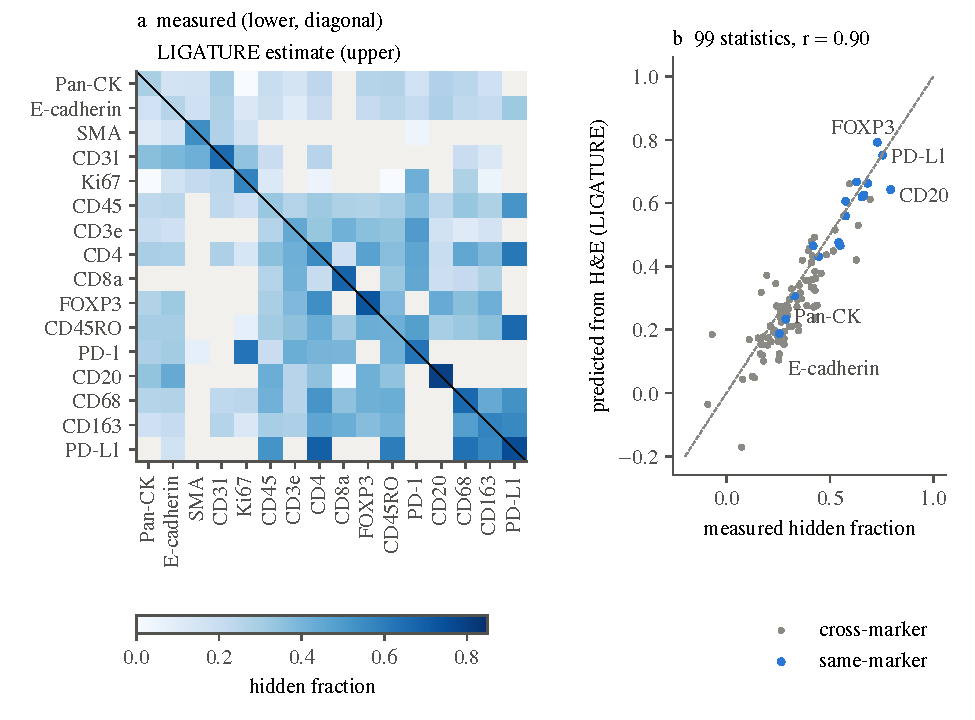
\includegraphics[width=\linewidth]{fig_hidden.pdf}
\caption{\textbf{a}, Fraction of each cohort-mean spatial statistic missing from the per-cell virtual stain, measured (lower triangle and diagonal) and estimated by \method{} from H\&E only on held-out patients (upper triangle); gray: $|$measured mean$|\le0.02$. \textbf{b}, Estimated against measured hidden fraction.}
\label{fig:hidden}
\end{figure}
\setcounter{section}{0}
\renewcommand{\thesection}{A\arabic{section}}

\section{Proofs}
\paragraph{Proposition~\ref{prop:bias}.} Write $Y=\mu+\varepsilon$ with $\E[\varepsilon\mid H]=0$. Then $Y_{ia}Y_{jb}=\mu_{ia}\mu_{jb}+\mu_{ia}\varepsilon_{jb}+\varepsilon_{ia}\mu_{jb}+\varepsilon_{ia}\varepsilon_{jb}$, and $\E[\cdot\mid H]$ of the two middle terms vanishes, so $\E[Q(Y)\mid H]=Q(\mu)+|E_w|^{-1}\sum_{i\ne j}w(d_{ij})\frac12(\Sigma_{ia,jb}+\Sigma_{ib,ja})$. Subtracting $Q(f)$ gives the claim. Nothing is assumed about $f$ beyond measurability with respect to $H$.

\paragraph{Proposition~\ref{prop:nonid}, cross-marker case.} With bivariate per-cell laws $\mathcal{N}(\mu_i,\Sigma_i)$, $\Sigma_i=\begin{psmallmatrix}\sigma_{ia}^2&\rho_i\sigma_{ia}\sigma_{ib}\\ \rho_i\sigma_{ia}\sigma_{ib}&\sigma_{ib}^2\end{psmallmatrix}$, any joint law of the $2n$ variables with these marginals has a correlation matrix in $\mathcal{F}=\{R\in\mathcal{E}_{2n}:R_{(i,a),(i,b)}=\rho_i\}$, a convex set, and every $R\in\mathcal{F}$ is attained by a Gaussian law with these marginals. $\E[Q\mid H]-Q(\mu)$ is linear in $R$, so its range is an interval with endpoints given by two semidefinite programs over $\mathcal{F}$. Non-Gaussian marginals restrict the attainable correlations further (Fr\'echet--Hoeffding bounds), so the Gaussian interval contains the interval for any marginals with the same means and variances whose copulas are unrestricted.

\paragraph{Proposition~\ref{prop:proper}.} (i) A bin-constant weight $w=\sum_k c_k\mathbf{1}_{B_k}$ gives $Q_{w,ab}=\sum_k c_k|E_k|\,G_{k,ab}/|E_w|$, which is linear in $S$ for fixed geometry. (ii) For each $j$, $\E\,\mathrm{CRPS}(F,\theta_j(S))$ is uniquely minimized over laws with finite mean at the true conditional law of $\theta_j(S)$ (strict propriety); a sum of such terms is minimized exactly when every term is, i.e.\ by any joint predictive law with the correct marginals along every $\theta_j$. The cell term identifies each per-cell marginal in the same way.

\paragraph{Proposition~\ref{prop:ident}.} (i) The hypothesis requires $f$ to reproduce the scored cell means, since a zero-mean residual cannot shift them; for a stain with region-mean error the hypothesis fails and a fit is a misspecified projection. Under the hypothesis, by Proposition~\ref{prop:proper}(ii) a minimizer's law of each scored coordinate equals the true conditional law, in particular its mean. Under the model $Y=f+R$ with $\E[R\mid H]=0$, the cross terms of $G_{k,ab}(f+R)$ vanish in expectation, so $\E[G_{k,ab}(Y)\mid H]=G_{k,ab}(f)+\Gamma_{k,ab}(\Sigma)$; equating means gives the identity. A bin-constant bilinear statistic is a linear combination of the $G_{k,ab}$ (Proposition~\ref{prop:proper}(i)), so its mean is also correct. (ii) Cell means do not depend on $\Sigma$, the mean of $G_{k,ab}$ depends on it only through $\Gamma_{k,ab}$, and contrasts and patient averages are linear in these. A perturbation $\Delta$ with $\Gamma_{k,ab}(\Delta)=0$ for all $k,a,b$ leaves all these means unchanged; an example is $\Delta_{ia,ib}=\Delta_{ib,ia}=\epsilon$ for one cell $i$ and $a\ne b$, which enters no bin because bins exclude $i=j$, and keeps $\Sigma+\Delta$ positive definite for small $\epsilon$ when $\Sigma$ is. It changes $\E[Y_{ib}\mid Y_{ia},H]=f_{ib}+\Sigma_{ib,ia}\Sigma_{ia,ia}^{-1}(Y_{ia}-f_{ia})$. The cell-level score constrains only the per-cell marginal variances $\Sigma_{ia,ia}$. Such perturbations still change the spread of scored statistics, through fourth moments, so they are weakly constrained by the full scores; they are not constrained by the means that determine point estimates.

\paragraph{Proposition~\ref{prop:alloc}.} (i) \[\partial_{\theta_k}\big[\mathrm{tr}(\Sigma_\theta^{-1}\Sigma^*)+\log\det\Sigma_\theta\big]=-\mathrm{tr}(\Sigma_\theta^{-1}K_k\Sigma_\theta^{-1}\Sigma^*)+\mathrm{tr}(\Sigma_\theta^{-1}K_k)=-\mathrm{tr}\big(\Sigma_\theta^{-1}K_k\Sigma_\theta^{-1}(\Sigma^*-\Sigma_\theta)\big),\] which vanishes at an interior KL projection; and with a frozen mean equal to the true conditional mean, $\E^*[Q_{W}(Y)]-\E_\theta[Q_{W}(Y)]=\mathrm{tr}\big(W(\Sigma^*-\Sigma_\theta)\big)$. These are the likelihood and moment equations of classical variance-component estimation; the statistic score chooses the moments to be the analyzed statistics. (ii) With $\Sigma^*=I+\rho A$ ($A$ the bin-1 adjacency) and $\Sigma=s^2I+c^2\mathbf{1}\mathbf{1}^\top$, whose eigenvalues are $\lambda_1=s^2+nc^2$ on $\mathbf{1}$ and $\lambda_0=s^2$ on its complement, the KL projection minimizes $\mathrm{tr}(\Sigma^{-1}\Sigma^*)+\log\det\Sigma=a/\lambda_1+(n-a)/\lambda_0+\log\lambda_1+(n-1)\log\lambda_0$ with $a=\mathbf{1}^\top\Sigma^*\mathbf{1}/n=1+2\rho N_1/n$. The minimizer is $\lambda_1=a$, $\lambda_0=(n-a)/(n-1)$, so for $\rho\ge0$ $c^2=(\lambda_1-\lambda_0)/n=2\rho N_1/(n(n-1))=\rho N_1/\binom n2$ (for $\rho<0$ the constrained optimum is $c^2=0$) and $s^2+c^2=\lambda_0+(\lambda_1-\lambda_0)/n=1$. The bin-1 moment has mean $\Gamma_1=c^2$ under the class and $\rho$ under the truth, so matching it gives $c^2=\rho$. We confirmed the closed form by numerical KL minimization on random neighbor graphs.

\paragraph{Proposition~\ref{prop:deff}.} $\Var(\bar Q)=m^{-2}\sum_{c,c'}\Cov(Q_c,Q_{c'})$. With equal variances $v$ and average correlation $\bar\rho$ over ordered pairs $c\ne c'$, this is $m^{-1}v(1+(m-1)\bar\rho)$, versus $m^{-1}v$ under independence.

\paragraph{Proposition~\ref{prop:conf}.} Given in the main text. Ties are handled by the infimum over a right-continuous step function; the bound does not require independence across statistics within a patient.

\begin{table}[htp]
\centering
\caption{Reference patient roles: four-run aggregate versus the direct reseed mean on 40 ORION patients. Each metric averages the per-run patient-MSE ratio; this is not prediction ensembling. LIGATURE uses the reference plus three current-code reseeds; direct prediction uses three seeds. Brackets are 95\% patient-bootstrap intervals conditional on fitted models (2,000 replicates); the final row is a paired difference, with positive values favoring direct prediction.}
\label{tab:primaryseeds}
\begin{tabular}{@{}>{\raggedright\arraybackslash}p{1.7in}ccc>{\raggedright\arraybackslash}p{1.1in}@{}}
\toprule
Estimator (runs) & MSE all & MSE cross & MSE same & range: all; same \\
\midrule
Global rescale (1) & \shortstack{0.89\\{}[0.83, 1.02]} & \shortstack{0.90\\{}[0.83, 1.05]} & \shortstack{0.83\\{}[0.76, 0.89]} & -- \\
Direct graph (stain inputs), reseed mean (3) & \shortstack{0.88\\{}[0.85, 0.95]} & \shortstack{0.92\\{}[0.88, 0.98]} & \shortstack{0.64\\{}[0.59, 0.68]} & 0.867--0.892; 0.629--0.655 \\
\method{} four-run aggregate (4) & \shortstack{0.91\\{}[0.87, 1.02]} & \shortstack{0.95\\{}[0.92, 1.06]} & \shortstack{0.61\\{}[0.55, 0.75]} & 0.883--0.945; 0.596--0.630 \\
\midrule
\method{} $-$ direct & \shortstack{+0.03\\{}[+0.01, +0.11]} & \shortstack{+0.03\\{}[+0.02, +0.11]} & \shortstack{-0.03\\{}[-0.07, +0.10]} & \\
\bottomrule
\end{tabular}

\end{table}

\section{Implementation details}
\label{app:impl}
\paragraph{Crop selection and windows.} The supplied crop release (\url{https://huggingface.co/datasets/csmp-hub/orion-crc}) contains 3,337 segmentation-selected regions, not all cells of the original whole slides. The preprocessing examines every supplied crop, drops cells smaller than 40 pixels, excludes centroids within 48 pixels of a crop boundary, requires an assigned nucleus of at least 20 pixels, and removes duplicate cells in overlapping crop interiors. After these rules and feature availability, 3,331 crops contain retained cells; 3,323 have both near and far pairs. The crop geometry and these selection rules define the estimand. CellPlex uses a different whole-slide processing pipeline and fixed split; its cell count and scores are not directly comparable to this subset.

\paragraph{Features and folds.} PCA (128 components) is fitted on 60,000 cells sampled from training patients of each rotation; cell features are standardized with training statistics. Regions are 512$\times$512 crops at 0.325\,$\mu$m/pixel; all cells retained by quality control are used, and pairs are computed among cells of the same region.
\paragraph{\method{}.} A preliminary generator trained with one energy score on the full statistic vector left the attenuation unchanged ($-34\%$), which motivated per-statistic scoring. Transformer width 128, 3 layers, 4 heads, attention bias from 16 Gaussian radial basis functions of distance (centres 0--160\,$\mu$m, width 10\,$\mu$m). Loadings are per-cell outputs of a two-layer head ($p\times K$, $K=4\cdot4+8+4+4=32$), scaled by 0.3 at initialization. Fields and region latents are independent between regions; only the patient latent couples regions. Random Fourier features: 64 per field and region, frequencies $\mathcal{N}(0,\ell^{-2}I)$, redrawn for each realization. Conditional on these features, residual draws are Gaussian; integrating their randomness gives a finite-feature Gaussian mixture with the stated kernel covariance. The cell term uses a moment-matched Gaussian approximation; region and patient CRPS score the actual generated statistics. Gaussian marginal/likelihood statements refer to the ideal field or their specified Gaussian surrogate, not the integrated finite-feature likelihood. Batches: 4 patients $\times$ 4 regions, 16 joint samples. Variance calibration: Adam (learning rate 0.05, 4 epochs) on the seven log-scales with the network frozen. The 4-region patient average in training is a noisier target than the all-region average evaluated at test time; with 8 regions per patient at the same batch size, results were unchanged (MSE 0.90 vs 0.92 of the plug-in's, raw coverage 73\% vs 71\%). Field rank 8 left validation loss unchanged and was not adopted.
\paragraph{Analytic point forecasts.} These remove Monte Carlo error from the conditional mean without changing the model; substituting expected moments into a ratio is a separate approximation. For bilinear statistics, conditional means follow by replacing each product by $f_{ia}f_{jb}+\operatorname{Cov}(Y_{ia},Y_{jb}\mid H)$ and averaging with its bin weights. This integrates all latent and random-feature second moments without Monte Carlo error. The core release additionally returns these 832 expected coordinates. Reference and reseed results above retain their original 64-draw means; samples remain necessary for their predictive laws and nonlinear queries.

\paragraph{Direct contact model.} The direct graph model's backbone (frozen embeddings, the stain's per-cell predictions as inputs, the same cell-graph transformer, mean and max pooling with log cell count) predicts, per region and per cell, the 16 positive-cell fractions $\pi_a$ and the 256 conditional contact probabilities $c_{ab}$, each a logit-scale correction of the quantile-matched plug-in's (training-patient gates for the measured targets, validation-fitted gates for the plug-in), so predicted contacts $\pi_ac_{ab}$ never exceed predicted positives $\pi_a$. It is trained with Gaussian CRPS on these per-cell counts for regions and patient averages (15 epochs, early stopping on validation patients, three seeds); a patient's contact fraction is the ratio of its summed predicted counts. The target-matched variant adds an absolute-error loss on each patient's pooled contact fraction (weight 10) and early-stops on it; it is the stronger baseline. An unconstrained variant predicting numerators and denominators separately is worse (ORION 0.82, lung 0.95).
\paragraph{Lung cohort.} HEST-1k v1.3 Xenium samples NCBI856--NCBI884 of \citet{vannan2025} (20 samples, 19 patients; 0.2125\,$\mu$m/pixel H\&E aligned to the transcripts). Transcripts with quality $\ge20$ assigned to a Xenium cell are counted per gene; each cell is placed at the centroid of the nearest Xenium cell polygon (within 8\,$\mu$m), whose area, perimeter and eccentricity are the morphology inputs, so no transcript-derived quantity enters the inputs. Targets are counts scaled to the median library size (cells with $\ge10$ transcripts). Genes: EPCAM, SFTPC, AGER, SCGB1A1, KRT5 (epithelial); PTPRC, CD3E, CD8A, MS4A1, CD68, MARCO, SPP1 (immune); COL1A1, ACTA2 (stromal); PECAM1 (endothelial); MKI67. Regions are 166.4\,$\mu$m squares with at least 40 cells, 80 per sample; Phikon-v2 embeddings use the same 20.8\,$\mu$m field of view (98 pixels). All model and training settings are those of ORION; contact statistics use the same 85th-percentile gates.

\paragraph{Virtual stains.} \emph{Transformer}: same architecture without noise, per-cell squared loss, 25 epochs, early stopping on validation patients. \emph{Ridge}: closed form on standardized cell features, penalty from $\{10,\dots,10^6\}$ by validation MSE. \emph{U-Net}: five-level encoder--decoder (32--384 channels) on H\&E downsampled to 0.65\,$\mu$m/pixel, pixel MSE plus per-cell MSE after mask pooling with a learned per-channel affine map, 40 epochs, early stopping on validation cell MSE. \emph{ROSIE}: released ConvNeXt-Small weights, loaded with a restricted unpickler; one 148-pixel patch per cell centroid (48\,$\mu$m, assuming 0.377\,$\mu$m/pixel for ROSIE's training images), resized to 224, ImageNet normalization; one affine map per marker from the matched channel, fitted on training patients. \emph{GigaTIME}: the released nested U-Net, re-implemented from the authors' description and loaded tensors-only; regions resized to 336$\times$336 ($\approx$0.5\,$\mu$m/pixel), per-pixel probabilities averaged over each cell mask; a ridge head on the 21 channel logits per marker, penalty chosen on validation patients. \emph{GigaTIME fine-tuned}: the same network with its output layer replaced by 16 channels (rows of matched markers initialized from GigaTIME's), trained end to end with the U-Net's loss, AdamW (learning rate $3\times10^{-4}$, one-cycle schedule), 30 epochs, best validation cell MSE. Table~\ref{tab:pubmarkers} reports per-cell transfer.

\begin{table}[htp]
\centering
\caption{Per-cell Pearson correlation between published-model predictions and measured ORION intensities on test patients (mean over rotations). GigaTIME is shown for markers with a matched channel.}
\label{tab:pubmarkers}
\normalsize
\begin{tabular}{@{}lcc@{}}
\toprule
Marker & ROSIE & GigaTIME \\
\midrule
CD163 & 0.15 & -- \\
CD20 & 0.25 & 0.22 \\
CD31 & 0.19 & -- \\
CD3e & 0.28 & 0.28 \\
CD4 & 0.18 & 0.32 \\
CD45 & 0.36 & -- \\
CD45RO & 0.37 & -- \\
CD68 & 0.17 & 0.24 \\
CD8a & 0.21 & 0.21 \\
E-cadherin & 0.14 & -- \\
FOXP3 & 0.12 & -- \\
Ki67 & 0.08 & 0.43 \\
PD-1 & 0.22 & 0.30 \\
PD-L1 & 0.24 & 0.24 \\
Pan-CK & 0.25 & 0.63 \\
SMA & 0.14 & -- \\
\bottomrule
\end{tabular}

\end{table}

\section{Additional results}

\begin{table}[t]
\centering
\caption{\method{} wrapped around six virtual stains (40 held-out patients). Cell MSE: per-cell test MSE of the stain. Bias: median relative bias of cohort means. MSE: patient-level MSE relative to the stain's own plug-in for all statistics and the 16 clustering statistics. CRPS: ratio to a calibrated Gaussian plug-in. Contact: patient-level MSE of gated contact fractions relative to the plug-in, for the quantile-matched plug-in and \method{}. $^\dagger$GigaTIME: bias, MSE and CRPS columns use the 45 statistics among the 9 markers it measures directly; contact uses all pairs, with other markers predicted by its linear head.}
\label{tab:stains}
\setlength{\tabcolsep}{3pt}
\begin{tabular}{@{}lcccccccc@{}}
\toprule
 & cell & \multicolumn{2}{c}{bias} & \multicolumn{2}{c}{MSE / plug-in} & CRPS & \multicolumn{2}{c}{contact MSE} \\
\cmidrule(lr){3-4}\cmidrule(lr){5-6}\cmidrule(lr){8-9}
Virtual stain & MSE & plug-in & \method{} & all & same & \method{}/Gauss. & quant. & \method{} \\
\midrule
Cell-graph transformer & 0.78 & $-34\%$ & $-6\%$ & 0.88 & 0.60 & 0.84 & 0.88 & 0.62 \\
Per-cell ridge, no context & 0.85 & $-39\%$ & $-2\%$ & 0.86 & 0.64 & 0.84 & 0.83 & 0.72 \\
Pixel U-Net & 0.78 & $-12\%$ & $+3\%$ & 1.04 & 0.84 & 0.90 & 0.94 & 0.62 \\
ROSIE & 1.04 & $-94\%$ & $+5\%$ & 0.61 & 0.45 & 0.66 & 1.71 & 0.47 \\
GigaTIME$^\dagger$ & 0.95 & $-68\%$ & $-6\%$ & 0.73 & 0.52 & 0.72 & 0.63 & 0.40 \\
GigaTIME fine-tuned & 0.78 & $-7\%$ & $+8\%$ & 0.96 & 0.81 & 0.89 & 0.94 & 0.67 \\
\bottomrule
\end{tabular}

\end{table}


\subsection{Additional gates and unscored query families}
\label{app:families}
The advantage holds at 75th- and 95th-percentile gates (contact error 0.83 and 0.43 vs 1.09 and 0.91 for the quantile-matched plug-in). Three further families behave similarly (Appendix Fig.~\ref{fig:downstream}a): near-minus-far co-positivity (MSE 0.70 of the plug-in's), products at radii finer than the training bins (attenuation 39\% to 10\%; MSE 0.91), and positive-cell fractions (MSE 0.88, but bias $+11\%$ vs $+5\%$ for the quantile-matched plug-in, a tail limit of the Gaussian residual).

\subsection{Empirical rationale and identification analysis}
\label{app:diagnostics}
The identification calculations use Gaussian marginals matched to the model's per-cell means and variances and bound conditional expectations over their admissible couplings. For non-Gaussian marginals the same semidefinite programs give moment-based outer bounds; endpoint attainability with fixed non-Gaussian marginals is not asserted. Comparisons with realized assay statistics provide empirical context; they do not validate predictive coverage or identify an individual tissue's molecular configuration.

\paragraph{Plug-in attenuation.}
Across the 136 statistics, the plug-in underestimates the cohort-mean statistic by a median of 34\% (30\% for cross-marker and 58\% for same-marker statistics; Fig.~\ref{fig:main}a, Table~\ref{tab:main}). The direction matches Proposition~\ref{prop:bias}: positive residual covariance between neighboring cells, which the per-cell mean cannot express, is missing (Fig.~\ref{fig:overview}). The errors are not independent across regions: the plug-in error of a region statistic has a median within-patient intraclass correlation of 0.087 (interquartile range 0.057--0.107), a median design effect of 6.4 at 63 regions per patient (Proposition~\ref{prop:deff}). Per-statistic calibration removes the cohort-mean bias on validation patients but transfers poorly: its patient-level MSE is 13\% \emph{higher} than the plug-in's and its rank correlation with the measured values is lower (0.41 vs 0.52), because affine corrections fitted on 8 patients do not transfer across patients.

\paragraph{What the stain does not capture.} The fraction of a cohort-mean statistic missing from the stain ranges on ORION from 11--15\% (epithelial--stromal segregation) to 66--79\% (immune and vascular clustering; Appendix Fig.~\ref{fig:hidden}), and \method{} estimates it from H\&E on held-out patients ($r=0.90$ across 99 statistics).

\paragraph{Identification from model-implied marginals.}
We computed Proposition~\ref{prop:nonid}'s interval for every same-marker statistic in 400 held-out regions (10 per test patient), using Gaussian marginals matched to \method{}'s calibrated per-cell means and variances. The solver is certified (dual gap at most 0.33\% at upper and 4.9\% at lower endpoints; Appendix). Patient-level intervals (the average of region intervals, since couplings across regions are unconstrained) bound the conditional expectation; they contain the measured value for 97\% of patient--marker pairs (all within two standard errors of the 10-region average) but are uninformative: their median width is 2.4 times the 5--95\% range of the statistic across the 40 patients and exceeds it for 14 of 16 markers (all but Pan-CK and E-cadherin clustering). The extremes are attained by sign-pattern couplings that real tissue need not exhibit, so we also restricted the coupling to stationary, nonnegative correlations decaying with distance. The restricted interval is narrower (median 0.64 of the cohort range) and, allowing for sampling error, consistent with the data (3.6\% of measured values lie more than two standard errors outside it), yet it still spans most of the between-patient range. Per-cell predictive laws thus leave spatial statistics largely undetermined unless the dependence is assumed or, as in \method{}, learned.


\begin{table}[htp]
\centering
\caption{Per-marker identification intervals for clustering statistics (patient level). Cohort range: 5--95\% range of the measured statistic across patients. Per-cell interval: width of Proposition~\ref{prop:nonid}'s interval from calibrated per-cell laws; restricted: stationary, nonnegative, decaying correlations. Ratios are to the cohort range.}
\label{tab:ident}
\normalsize
\begin{tabular}{@{}lrrrrrr@{}}
\toprule
Marker & cohort & \method{} & per-cell & ratio & restricted & ratio \\
\midrule
E-cadherin & 0.55 & 0.30 & 0.34 & 0.6 & 0.09 & 0.17 \\
Pan-CK & 0.46 & 0.29 & 0.38 & 0.8 & 0.10 & 0.22 \\
CD20 & 0.65 & 0.21 & 0.84 & 1.3 & 0.22 & 0.34 \\
Ki67 & 0.46 & 0.31 & 0.86 & 1.9 & 0.23 & 0.51 \\
CD4 & 0.61 & 0.26 & 1.19 & 1.9 & 0.32 & 0.52 \\
CD45 & 0.40 & 0.27 & 0.82 & 2.0 & 0.21 & 0.53 \\
CD8a & 0.47 & 0.22 & 0.95 & 2.0 & 0.27 & 0.58 \\
CD45RO & 0.39 & 0.20 & 0.91 & 2.3 & 0.24 & 0.62 \\
CD31 & 0.34 & 0.28 & 0.84 & 2.4 & 0.23 & 0.66 \\
CD3e & 0.43 & 0.25 & 1.30 & 3.0 & 0.35 & 0.81 \\
PD-L1 & 0.21 & 0.12 & 0.66 & 3.2 & 0.17 & 0.82 \\
SMA & 0.35 & 0.27 & 1.24 & 3.6 & 0.31 & 0.89 \\
CD163 & 0.34 & 0.34 & 1.24 & 3.7 & 0.32 & 0.95 \\
PD-1 & 0.23 & 0.20 & 0.95 & 4.1 & 0.25 & 1.07 \\
FOXP3 & 0.16 & 0.16 & 0.68 & 4.3 & 0.19 & 1.19 \\
CD68 & 0.28 & 0.21 & 1.22 & 4.4 & 0.32 & 1.14 \\
\bottomrule
\end{tabular}

\end{table}

\begin{table}[htp]
\centering
\caption{Coverage of patient-level intervals by rotation (all 136 statistics).}
\label{tab:perfold}
\normalsize
\begin{tabular}{@{}lccccc@{}}
\toprule
Rotation & raw 90\% & inflated & conformal & $\hat\tau$ infl. & $\hat\tau$ conf. \\
\midrule
0 & 0.87 & 0.94 & 0.98 & 1.33 & 2.84 \\
1 & 0.67 & 0.87 & 0.95 & 1.57 & 3.30 \\
2 & 0.74 & 0.92 & 0.99 & 1.73 & 3.88 \\
3 & 0.70 & 0.96 & 0.99 & 2.32 & 5.51 \\
4 & 0.74 & 0.86 & 0.95 & 1.53 & 3.74 \\
\bottomrule
\end{tabular}

\end{table}

\begin{table}[htp]
\centering
\caption{Hybrid inference with measured anchor markers: patient-level MSE relative to the anchor-substituted plug-in, statistics involving at least one unmeasured marker.}
\label{tab:hybrid}
\normalsize
\begin{tabular}{@{}l>{\centering\arraybackslash}p{.8in}>{\centering\arraybackslash}p{1.35in}>{\centering\arraybackslash}p{.8in}>{\centering\arraybackslash}p{1.1in}c@{}}
\toprule
Anchors & ridge imput. & \method{}, substituted & exact cond. & regularized cond. & $\delta$ \\
\midrule
Pan-CK, CD45 & 1.07 & 0.90 & 1.36 & 0.95 & 1 \\
PD-L1, CD8a & 1.30 & 0.87 & 3.96 & 1.28 & 1 \\
CD3e & 1.17 & 0.88 & 1.47 & 0.94 & 1 \\
\bottomrule
\end{tabular}

\end{table}

\begin{table}[htp]
\centering
\caption{Gated contact fractions for selected pairs across virtual stains: patient-level MSE relative to each stain's plug-in, quantile-matched plug-in / \method{}. Over all pairs, wrapping the ridge stain gives the same ordering (MSE 1.00, 0.83, 0.72; $\rho$ 0.47, 0.50, 0.56).}
\label{tab:contactex}
\normalsize
\begin{tabular}{@{}lccccc@{}}
\toprule
Pair & transformer & ridge & U-Net & ROSIE & GigaTIME \\
\midrule
CD8a $\to$ Pan-CK & 0.99 / 0.60 & 0.57 / 0.52 & 0.88 / 0.68 & 2.60 / 0.43 & 0.67 / 0.32 \\
CD3e $\to$ Pan-CK & 0.82 / 0.43 & 0.37 / 0.41 & 0.67 / 0.51 & 6.11 / 0.71 & 0.85 / 0.40 \\
CD68 $\to$ PD-L1 & 1.03 / 0.51 & 1.27 / 0.93 & 1.64 / 0.55 & 1.02 / 0.39 & 0.83 / 0.41 \\
PD-L1 $\to$ CD8a & 1.09 / 0.96 & 0.72 / 0.93 & 0.71 / 0.64 & 0.28 / 0.46 & 0.55 / 0.66 \\
FOXP3 $\to$ CD8a & 1.09 / 0.80 & 0.46 / 0.69 & 0.55 / 0.68 & 0.74 / 0.83 & 0.45 / 0.70 \\
CD8a $\to$ CD68 & 0.69 / 0.33 & 0.32 / 0.18 & 0.81 / 0.39 & 0.14 / 0.08 & 0.23 / 0.09 \\
\bottomrule
\end{tabular}

\end{table}

\begin{table}[htp]
\centering
\caption{Cellular-neighborhood composition across virtual stains (40 held-out patients): mean total-variation distance between predicted and measured per-patient frequencies of 10 neighborhoods, Wilcoxon $p$ and number of patients for which \method{}-Q is closer than the quantile-matched plug-in, and mean per-neighborhood rank correlation across patients (k-means is fitted per rotation; clusters are aligned to the first rotation's by Hungarian matching of centroids before pooling). GigaTIME markers without a matched channel come from its linear head.}
\label{tab:cn}
\normalsize
\begin{tabular}{@{}lcccccccc@{}}
\toprule
 & \multicolumn{4}{c}{total variation to measured} & & & \multicolumn{2}{c}{rank corr.} \\
\cmidrule(lr){2-5}\cmidrule(lr){8-9}
Virtual stain & plug-in & quant. & \method{} & \method{}-Q & $p$ & better & quant. & \method{}-Q \\
\midrule
Cell-graph transformer & 0.42 & 0.34 & 0.36 & 0.29 & 0.005 & 26/40 & 0.52 & 0.57 \\
Per-cell ridge & 0.54 & 0.33 & 0.42 & 0.29 & 0.006 & 27/40 & 0.54 & 0.54 \\
Pixel U-Net & 0.44 & 0.34 & 0.36 & 0.28 & 0.002 & 30/40 & 0.54 & 0.55 \\
ROSIE & 0.72 & 0.54 & 0.46 & 0.36 & $4.6{\times}10^{-10}$ & 36/40 & 0.18 & 0.36 \\
GigaTIME & 0.69 & 0.40 & 0.44 & 0.32 & $3.8{\times}10^{-5}$ & 32/40 & 0.37 & 0.43 \\
GigaTIME fine-tuned & 0.49 & 0.36 & 0.42 & 0.29 & $5.7{\times}10^{-4}$ & 29/40 & 0.51 & 0.51 \\
\bottomrule
\end{tabular}

\end{table}

\begin{table}[htp]
\centering
\caption{Empirical bias identity on test patients. For residual $r=y-f$, each binned moment satisfies $G(y)=G(f)+G(r)+X(f,r)$; $G(r)$ is the residual second moment (Proposition~\ref{prop:bias}'s covariance term plus the stain's mean-error term $G(\delta)$, $\delta=\mu-f$) and $X$ the predictor--residual cross term, zero in expectation when $f$ is the conditional mean $\mu$. Columns: median over the statistics with $|$measured cohort mean$|>0.02$ (99 on ORION, 62 on the lung cohort) of the plug-in's relative bias and of each term's cohort mean relative to the measured cohort mean; share of statistics with negative cross term; median per-patient root-mean-square of each term relative to the between-patient standard deviation. GigaTIME is evaluated here on all 136 statistics (other markers from its linear head), so its bias differs from Table~\ref{tab:stains}.}
\label{tab:biasdec}
\normalsize
\begin{tabular}{@{}lcccccc@{}}
\toprule
 & plug-in & \multicolumn{3}{c}{cohort mean / measured} & \multicolumn{2}{c}{per-patient RMS / s.d.} \\
\cmidrule(lr){3-5}\cmidrule(lr){6-7}
Virtual stain & bias & $G(r)$ & $X(f,r)$ & $X<0$ & $G(r)$ & $X(f,r)$ \\
\midrule
Cell-graph transformer & $-34\%$ & $+31\%$ & $+3\%$ & 39\% & 0.47 & 0.64 \\
Per-cell ridge & $-39\%$ & $+42\%$ & $-2\%$ & 61\% & 0.60 & 0.65 \\
Pixel U-Net & $-12\%$ & $+34\%$ & $-19\%$ & 93\% & 0.53 & 0.70 \\
ROSIE & $-94\%$ & $+90\%$ & $-2\%$ & 54\% & 1.09 & 0.34 \\
GigaTIME & $-59\%$ & $+71\%$ & $-14\%$ & 84\% & 0.89 & 0.60 \\
GigaTIME fine-tuned & $-7\%$ & $+36\%$ & $-25\%$ & 88\% & 0.56 & 0.75 \\
\midrule
Lung (Xenium), transformer & $-71\%$ & $+64\%$ & $+4\%$ & 32\% & 0.74 & 0.57 \\
\bottomrule
\end{tabular}

\end{table}

\paragraph{Empirical bias identity.} With $r=Y-f$ and mean error $\delta=\mu-f$, every binned moment splits as $G(Y)=G(f)+G(r)+X(f,r)$, where $\E[G(r)\mid H]$ is the residual second moment, $G(\delta)$ plus Proposition~\ref{prop:bias}'s covariance term, and $\E[X(f,r)\mid H]=X(f,\delta)$ vanishes when $f=\mu$. On test patients (Table~\ref{tab:biasdec}) the residual second moment is similar for all in-domain stains (31--42\% of the measured statistic), but the cross term is near zero only for the transformer ($+3\%$; $+4\%$ on the lung cohort), the per-cell ridge and ROSIE (both $-2\%$). For the pixel-level stains it is negative ($-19\%$, $-25\%$): their mean error is anti-aligned with neighboring predictions and offsets the residual second moment, which a frozen-mean wrapper cannot undo.

\begin{table}[htp]
\centering
\caption{Patient-disjoint calibration on ORION (5 rotations, 40 test patients). Stain and generator are retrained on 20 patients per rotation; 2 patients serve model selection and variance fitting and 10 serve calibration only. Per-statistic split-conformal 90\% intervals (rank 10 of 10); width and interval score are normalized per statistic and averaged; calibration does not change point predictions (clustering MSE 0.66 of the matched plug-in's). Coverage is marginal per statistic, not simultaneous or patient-conditional; ORION was examined during development, so this is not a confirmatory cohort. An earlier exact version with only 4 calibration patients (wrapping ROSIE, whose maps use training patients only) was uninformative even at an 80\% target.}
\label{tab:indcal}
\normalsize
\begin{tabular}{@{}p{2.55in}cccccc@{}}
\toprule
 & \multicolumn{3}{c}{clustering (16)} & \multicolumn{3}{c}{all 136} \\
\cmidrule(lr){2-4}\cmidrule(lr){5-7}
Method & cov. & width & score & cov. & width & score \\
\midrule
\method{} samples, raw & 45.6\% & 1.06 & 6.37 & 70.4\% & 1.75 & 4.85 \\
\method{} + conformal & 90.0\% & 3.81 & 4.98 & 90.2\% & 3.59 & 4.86 \\
\method{} center, constant scale + conformal & 90.9\% & 3.77 & 5.22 & 90.9\% & 3.95 & 5.64 \\
plug-in, Gaussian (validation scale) & 74.7\% & 2.72 & 7.05 & 72.0\% & 2.39 & 6.78 \\
plug-in + conformal & 91.1\% & 4.63 & 6.69 & 91.5\% & 4.09 & 5.89 \\
global rescale + conformal & 92.3\% & 4.47 & 6.18 & 90.6\% & 4.88 & 7.13 \\
family rescale + conformal & 91.7\% & 4.40 & 6.09 & 90.8\% & 4.92 & 7.13 \\
rescale, \method{} scale + conformal & 92.3\% & 4.46 & 5.76 & 89.5\% & 4.17 & 5.67 \\
\bottomrule
\end{tabular}

\end{table}

\begin{table}[htp]
\centering
\caption{Patient-disjoint calibration of statistics never scored in training (same refit as Table~\ref{tab:indcal}; gates and neighborhood templates fitted on the 20 training patients, quantile-matched thresholds on the 2 selection patients, 10 calibration patients). Prespecified mean/SD conformal 90\% intervals; width and interval score in the statistic's units. Width and score differences from the quantile-matched plug-in are not statistically significant (descriptive paired intervals cross zero), and a constant-scale interval around \method{}-Q scores similarly; point error is 26\% (contacts) and 24\% (neighborhoods) below the quantile-matched plug-in's, as ratios of equal-patient mean squared errors (each patient's squared errors averaged over its eligible statistics, then patients averaged), not per-statistic normalized ratios as elsewhere; coverage, width and score also give patients equal weight; calibration does not change point estimates. Contact pairs require at least 20 measured positive source cells, an outcome-defined eligibility, and 25\% of adaptive contact intervals span all of $[0,1]$. A conformalized-quantile variant chosen after these results (a development diagnostic, not prespecified) narrows neighborhood intervals by 12\% relative to the quantile-matched plug-in (better in 38 of 40 patients).}
\label{tab:unscoredcal}
\normalsize
\begin{tabular}{@{}p{2.45in}cccccc@{}}
\toprule
 & \multicolumn{3}{c}{contact fractions} & \multicolumn{3}{c}{neighborhood frequencies} \\
\cmidrule(lr){2-4}\cmidrule(lr){5-7}
Method & cov. & width & score & cov. & width & score \\
\midrule
\method{}-Q samples, raw & 45.5\% & 0.247 & 1.656 & 44.3\% & 0.089 & 0.748 \\
\method{}-Q + conformal & 91.6\% & 0.646 & 0.808 & 92.8\% & 0.321 & 0.421 \\
\method{}-Q center, constant scale + conformal & 92.5\% & 0.642 & 0.798 & 92.2\% & 0.290 & 0.421 \\
\method{} + conformal & 91.4\% & 0.613 & 0.783 & 90.0\% & 0.316 & 0.447 \\
quantile-matched plug-in + conformal & 92.6\% & 0.653 & 0.819 & 90.0\% & 0.310 & 0.461 \\
plug-in + conformal & 91.9\% & 0.633 & 0.846 & 88.5\% & 0.311 & 0.478 \\
\bottomrule
\end{tabular}

\end{table}

\begin{table}[htp]
\centering
\caption{Patient-disjoint calibration on the lung cohort (5 rotations, 19 test patients): stain and generator retrained on 10--11 patients, 1 for model selection and variance fitting, 4 for calibration only. With 4 calibration patients a finite split-conformal interval exists only up to 80\%, so the target (fixed before fitting) is 80\% (rank 4 of 4), not 90\%. Per-fold clustering coverage ranges 65.6--90.6\%; the constant-scale control is narrower with a similar score, so adaptive spread shows no established advantage here; one selection patient makes rescaling baselines unstable. Development evidence; point MSE 0.49 (clustering) of the refit's matched plug-in.}
\label{tab:lungcal}
\normalsize
\begin{tabular}{@{}p{2.55in}cccccc@{}}
\toprule
 & \multicolumn{3}{c}{clustering (16)} & \multicolumn{3}{c}{all 136} \\
\cmidrule(lr){2-4}\cmidrule(lr){5-7}
Method & cov. & width & score & cov. & width & score \\
\midrule
\method{} samples, raw & 27.6\% & 0.57 & 4.78 & 50.2\% & 1.29 & 4.50 \\
\method{} + conformal & 82.6\% & 3.57 & 4.60 & 80.3\% & 3.38 & 4.84 \\
\method{} center, constant scale + conformal & 81.6\% & 3.05 & 4.60 & 80.1\% & 3.36 & 5.18 \\
plug-in, Gaussian (validation scale) & 55.9\% & 3.07 & 6.84 & 49.4\% & 1.71 & 5.95 \\
plug-in + conformal & 79.9\% & 4.44 & 6.77 & 79.6\% & 3.58 & 5.69 \\
global rescale + conformal & 79.3\% & 4.01 & 6.07 & 77.1\% & 4.39 & 7.59 \\
family rescale + conformal & 78.3\% & 4.13 & 6.52 & 78.2\% & 3.81 & 6.28 \\
rescale, \method{} scale + conformal & 80.6\% & 4.50 & 5.80 & 77.6\% & 4.42 & 6.58 \\
\bottomrule
\end{tabular}

\end{table}

\begin{table}[htp]
\centering
\caption{All estimators on one scale: patient-level MSE relative to the cell-graph transformer's plug-in, averaged over the 136 statistics (all) and the 16 clustering statistics (same), and mean Spearman correlation with measured values across 40 held-out patients. No stain: estimators that use only the cell embeddings. Learned mean correction: \method{} with a zero-initialized correction added to the frozen stain. Direct graph with stain inputs: the direct model given the stain's per-cell predictions, predicting a correction of the stain's plug-in statistics. Conditional Gaussian NLL: the backbone trained by the joint Gaussian likelihood of each region's cells (Woodbury form, one random-feature draw per region), early-stopped on validation likelihood, conditional on the sampled features, with a $0.01I$ cell-covariance nugget for invertibility that is absent from the sampler; this is not the integrated mixture likelihood. Results precede variance calibration (calibrating its scales by likelihood made it worse; on the lung cohort the fit was numerically unstable).}
\label{tab:common}
\normalsize
\begin{tabular}{@{}>{\raggedright\arraybackslash}p{.85in}>{\raggedright\arraybackslash}p{3.2in}ccc@{}}
\toprule
Stain & Estimator & MSE all & MSE same & $\rho$ \\
\midrule
No stain & Direct ridge on region features & 1.42 & 0.99 & 0.31 \\
 & Direct graph (no stain) & 1.30 & 0.91 & 0.38 \\
 & \method{} around a constant stain & 1.13 & 0.76 & 0.46 \\
 & \method{} around a constant stain, learned mean & 1.00 & 0.75 & 0.48 \\
\addlinespace
Transformer & plug-in & 1.00 & 1.00 & 0.52 \\
 & global rescale & 0.89 & 0.83 & 0.54 \\
 & Direct graph (stain inputs) & 0.89 & 0.63 & 0.53 \\
 & regularized conditional Gaussian NLL & 2.75 & 4.46 & 0.35 \\
 & \method{} & 0.88 & 0.60 & 0.53 \\
\addlinespace
Ridge & plug-in & 1.36 & 1.32 & 0.42 \\
 & \method{} & 1.13 & 0.78 & 0.42 \\
\addlinespace
U-Net & plug-in & 1.07 & 0.98 & 0.51 \\
 & \method{} & 1.09 & 0.76 & 0.47 \\
 & \method{}, learned mean correction & 1.03 & 0.72 & 0.48 \\
\addlinespace
ROSIE & plug-in & 2.37 & 2.37 & 0.18 \\
 & \method{} & 1.17 & 0.87 & 0.46 \\
\addlinespace
GigaTIME & plug-in & 1.80 & 1.86 & 0.28 \\
 & \method{} & 1.14 & 0.79 & 0.43 \\
 & \method{}, learned mean correction & 1.09 & 0.74 & 0.44 \\
\addlinespace
GigaTIME fine-tuned & plug-in & 1.12 & 0.95 & 0.51 \\
 & \method{} & 1.05 & 0.74 & 0.51 \\
 & \method{}, learned mean correction & 1.06 & 0.72 & 0.51 \\
\bottomrule
\end{tabular}

\end{table}

\begin{table}[htp]
\centering
\caption{Known-law simulations on ORION's cells, regions, patients and embeddings (40 patients, five held-out rotations). Targets are $Y=f^\star+R$ with $f^\star$ the fold-0 stain's predictions, so the plug-in of $f^\star$ is the Bayes per-cell predictor, and $R$ a member of \method{}'s class: exact squared-exponential fields at 20 and 80\,$\mu$m (rank 2) with embedding-dependent loadings, cell noise ($\sigma=0.6$) and a patient latent. The second case adds a shared cell-level factor (loading 0.6) to CD8a/Pan-CK and CD68/PD-L1, a within-cell cross-marker covariance with zero bin averages. \method{} is fitted to the simulated targets with the reference configuration and $f^\star$ as its frozen stain. \emph{Top}: patient-level MSE of the 136 contrasts relative to the plug-in and median relative bias; the Bayes statistic predictor adds the exact $\E[G(r)\mid H]$ under the simulated law to the plug-in. \emph{Bottom}: residual correlations on test cells, within a cell and between cells 0--25\,$\mu$m apart (normalized by within-cell variances), true and implied by \method{}'s loadings.}
\label{tab:sim}
\normalsize
\setlength{\tabcolsep}{2pt}
\begin{tabular}{@{}lcccccc@{}}
\toprule
 & \multicolumn{3}{c}{Correct model class} & \multicolumn{3}{c}{Within-cell dependence added} \\
\cmidrule(lr){2-4}\cmidrule(lr){5-7}
Contrast estimator & MSE all & MSE same & bias & MSE all & MSE same & bias \\
\midrule
Plug-in of the true mean & 1.00 & 1.00 & $-38\%$ & 1.00 & 1.00 & $-37\%$ \\
\method{} & 0.59 & 0.12 & $+1\%$ & 0.61 & 0.12 & $+2\%$ \\
Bayes statistic predictor & 0.32 & 0.07 & $-1\%$ & 0.33 & 0.07 & $0\%$ \\
\bottomrule
\end{tabular}

\medskip

\begin{tabular}{@{}lcccccccc@{}}
\toprule
 & \multicolumn{4}{c}{Correct model class} & \multicolumn{4}{c}{Within-cell dependence added} \\
\cmidrule(lr){2-5}\cmidrule(lr){6-9}
 & \multicolumn{2}{c}{within cell} & \multicolumn{2}{c}{0--25\,\textmu m} & \multicolumn{2}{c}{within cell} & \multicolumn{2}{c}{0--25\,\textmu m} \\
Residual correlation & true & \method{} & true & \method{} & true & \method{} & true & \method{} \\
\midrule
CD8a / Pan-CK & $-0.14$ & $-0.00$ & $-0.12$ & $-0.09$ & $+0.22$ & $+0.01$ & $-0.09$ & $-0.06$ \\
CD68 / PD-L1 & $+0.01$ & $-0.11$ & $-0.03$ & $-0.01$ & $+0.36$ & $-0.20$ & $-0.02$ & $-0.01$ \\
Other 118 pairs, mean abs.\ error & \multicolumn{2}{c}{0.12} & \multicolumn{2}{c}{0.02} & \multicolumn{2}{c}{0.12} & \multicolumn{2}{c}{0.01} \\
\bottomrule
\end{tabular}

\end{table}
\begin{table}[htp]
\centering
\caption{Fixed-model same-marker sensitivity to immediately neighboring supplied cell masks (40 patients, 16 markers). Both variants use the same \ControlRegions{} regions, equal-region patient averages and each variant's own plug-in denominator. LIGATURE predictions integrate the model's second moments analytically, including random Fourier features; they are not the stored 64-draw mean used in Table~\ref{tab:main}. Intervals are 95\% patient bootstraps conditional on the fixed models (2,000 replicates). Bias is the median signed relative cohort-mean error across the 16 markers with measured mean magnitude above 0.02.}
\label{tab:segmentation}
\begin{tabular}{@{}lccc@{}}
\toprule
Near-pair rule & MSE / plug-in [95\% interval] & Plug-in bias & LIGATURE bias \\
\midrule
All near pairs & 0.60 [0.54, 0.72] & $-58\%$ & $-5\%$ \\
Non-touching masks & 0.72 [0.62, 1.07] & $-53\%$ & $+6\%$ \\
\bottomrule
\end{tabular}

\end{table}

\paragraph{Mask-exclusion protocol.} Before computing sensitivity metrics, we fixed the rule in the released analysis plan: exclude near pairs if pixels in their supplied whole-cell masks have Chebyshev distance at most two pixels (0.65\,$\mu$m along an axis); keep the far bin unchanged. This removes \ControlRemovedPairs{} of \ControlInitialPairs{} undirected near pairs (\ControlRemovedPercent\%) and leaves \ControlRetainedPairs{}. Distance bins use the original stored masks, avoiding threshold changes from float32 distance rounding. One originally eligible region has no retained near pairs and is excluded from both diagnostic variants. The stain and generator are unchanged, with each patient's original held-out model; no control-specific training or threshold tuning occurs. Conditional expected products are $f_{ia}f_{ja}+\hat\Sigma_{ia,ja}$, integrated over the sampled Gaussian fields and their random Fourier features. A 1,024-draw check on the first held-out region agrees within Monte Carlo uncertainty. The restricted target differs from the original statistic. This is a post-development sensitivity check, not intensity-spillover correction, a segmentation benchmark or a claim that remaining dependence is biological.

\clearpage
\begin{figure}[!htp]
\centering
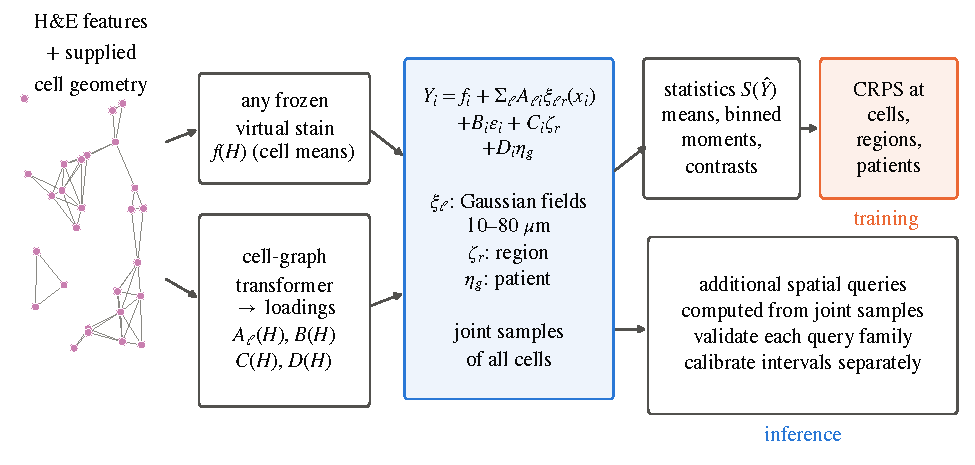
\includegraphics[width=\linewidth]{fig_schematic.pdf}
\caption{\method{} maps a frozen stain and cell features to a joint residual distribution, trained by CRPS on cell markers, region statistics and patient averages. Shared patient latents couple samples across regions. Primary geometry is supplied by the assay segmentation; additional computed queries require separate validation, and their intervals require query-specific calibration. An illustrative held-out region is shown in Appendix Fig.~\ref{fig:maps}.}
\label{fig:modeldiagram}
\end{figure}
\clearpage
\section{Additional rationale and diagnostic commentary}
\begin{proposition}[Likelihood versus statistic scoring]\label{prop:alloc}
Let a residual model have covariance $\Sigma_\theta=\sum_k\theta_kK_k$ with fixed positive semidefinite components $K_k$ (cell noise, fields at fixed scales, latents) and let the truth be $\Sigma^*$. (i) At an interior optimum, the Gaussian-likelihood projection satisfies $\mathrm{tr}\big(\Sigma_\theta^{-1}K_k\Sigma_\theta^{-1}(\Sigma^*-\Sigma_\theta)\big)=0$ for every free $\theta_k$, whereas, for a frozen mean equal to the true conditional mean, a fit reproducing the means of the analyzed bilinear statistics $Q_{W_j}$ solves $\mathrm{tr}\big(W_j(\Sigma^*-\Sigma_\theta)\big)=0$ for every $j$: a $\Sigma^*$ in the class satisfies both sets of equations, without implying uniqueness for the statistic equations; under misspecification likelihood weighs covariance errors by the whitened component designs and statistic scores by the analysis weights. (ii) For a positive-definite unit-variance covariance with correlation $\rho\ge0$ on the $N_1$ cell pairs of bin $B_1$, fitted with $\{I,\mathbf{1}\mathbf{1}^\top\}$, likelihood gives region-latent variance $c^2=\rho N_1/\binom{n}{2}$, attenuating the bin-1 covariance by the fraction of pairs outside $B_1$, and the bin-1 statistic gives $c^2=\rho$.
\end{proposition}

In ORION the plug-in errors of the 136 region statistics have a median within-patient intraclass correlation of 0.087 (interquartile range 0.057--0.107); with a median of 63 regions per patient and this ICC as a proxy for $\bar\rho$, the median design effect is about 6, so region-independent uncertainty would understate patient-level variance several-fold. \method{} therefore shares a patient latent across regions and scores patient averages of the statistics, for which Proposition~\ref{prop:proper} applies unchanged.


\subsection{Downstream checks}
\emph{Association studies.} For the 36 pairs of nine predefined spatial biomarkers, we estimated across-patient Spearman correlations as a virtual-population study would (Appendix Fig.~\ref{fig:downstream}b). \method{}, recomputing each correlation per joint sample, has mean absolute error 0.099 versus 0.149 for the plug-in; the difference is not statistically significant with 40 patients (bootstrap 90\% interval for the reduction $-2\%$ to 40\%, including zero); its intervals cover the measured correlation for 83\% of pairs versus 78\% for Fisher intervals on the plug-in.

\emph{Which patients to measure.} Measuring the 20\% of patients with the widest predictive distribution removes 50\% of the cohort's squared error (random 20\%, oracle 80\%; Appendix Fig.~\ref{fig:downstream}c), but, as reported for virtual transcriptomics \citep{batique2026}, this signal is mostly carried by the predicted value: ranking by the magnitude of the plug-in statistic removes 51\%, and the part of the spread not explained by \method{}'s predicted magnitude has partial rank correlation 0.18 with the error (28\% removed). Predictive spread adds little triage information beyond the predicted magnitude here.


\subsection{Ablation detail}
Systematic ablations (36 variants of five rotations on both cohorts; Appendix Table~\ref{tab:ablationfull}) separate what matters. The three current-code reseeds have MSE $\SeedMSEMean\pm\SeedMSESD$ (range \SeedMSEMin--\SeedMSEMax; clustering 0.60--0.63), with raw coverage $\SeedCoverageMean\pm\SeedCoverageSD\%$ (range \SeedCoverageMin--\SeedCoverageMax\%); small ablation differences should be assessed against this observed variation. The rerotation, with the stain retrained, gives 0.93 (clustering 0.64; per-patient Wilcoxon $p=0.07$ and $5\times10^{-6}$ against the plug-in), median bias $-34\%\to-5\%$, while the direct graph (stain inputs) has 0.91 overall and 0.69 for clustering. Essential: statistic-level scores (scored per cell only, as in engression-style generators \citep{engression2024}, MSE \CurrentCellOnlyMSE{} with current code versus \OldCellOnlyMSE{} in the earlier Table~\ref{tab:ablation} run; lung 2.27), scoring the bin contrasts (1.29 without), morphology-dependent loadings (stationary: clustering 0.67, raw coverage 39\%) and the patient latent (current raw coverage \CurrentNoPatientCoverage\% without; earlier run \NoPatientCoverage\%). Spatial fields reduce overall error (\CurrentNoFieldsMSE{} without them with current code, \OldNoFieldsMSE{} in the earlier run; lung 0.94 vs 0.84--0.86), but without them ORION clustering (0.62) and CRPS (0.0282) stay within seed variation, with smaller bias magnitude ($+2\%$) and higher raw coverage (82\%). Within noise: any one statistic-level score, the region latent, the number of field scales or their rank, network depth, morphology descriptors, the stain as residual-network input, and 6 rather than 24 training patients; a narrower network or 5 epochs scored at the favorable edge, so the reference is not tuned to its limit. Independently sampled Gaussian per-cell residuals with fitted marginal variances leave the attenuation unchanged and cover 28\% (Table~\ref{tab:ablation}), as Proposition~\ref{prop:nonid} predicts.


\clearpage
\begin{table}[!htp]
\centering
\caption{ORION evaluation labels used throughout. Patient roles are training/validation/test for 24/8/8, and training/selection/calibration/test for 20/2/10/8. Runs (L/D) count \method{}/direct fits per rotation for the scored-statistic head; new-query direct heads are fitted separately. MSE is overall patient-level MSE relative to that evaluation's plug-in. Reseed variation is sample SD. The four-run aggregate combines the reference run with three reseeds; its paired direct comparison uses the direct reseed mean. Independent calibration and H\&E geometry are separate evaluations; H\&E geometry also changes the cell-proxy target.}
\label{tab:runregistry}
\begin{tabular}{@{}lcccc@{}}
\toprule
Evaluation & Patient roles & Runs (L/D) & \shortstack{\method{}\\MSE} & \shortstack{Direct graph\\MSE} \\
\midrule
Reference run & 24/8/8 & 1/1 & 0.88 & 0.89 \\
Reseed mean & 24/8/8 & 3/3 & 0.92$\pm$0.02 & 0.88 \\
Four-run aggregate & 24/8/8 & 4/-- & 0.91 & -- \\
Rerotation & 24/8/8 & 1/1 & 0.93 & 0.91 \\
Independent calibration & 20/2/10/8 & 3/3 & 0.95 & 0.96 \\
H\&E geometry & 20/2/10/8 & 1/1 & 0.96 & 0.93 \\
\bottomrule
\end{tabular}

\end{table}

\section{Matched forecast, query-reuse and geometry checks}
\label{app:querybench}

\paragraph{Fixed protocol and scope.} These follow-up experiments use the five independent-calibration rotations (20 training, 2 selection, 10 calibration and 8 test patients). Training/selection features and the frozen stains reproduce that refit. Seeds 271027, 272027 and 273027 are fixed for the residual generators and direct heads; the first generator seed is reused. Stains are fixed across these seeds, so this does not measure full-pipeline seed variability. Global/family rescaling fitted on the two selection patients is unstable here (overall MSE ratios 1.85/1.84), unlike the eight-validation-patient reference protocol. The direct models use the same transformer inputs, stain predictions, width/depth, region/patient CRPS, 15 epochs and selection rule. One head predicts all 832 scored coordinates; another jointly predicts the 48 new-query coordinates. No calibration or test labels enter model fitting, early stopping, variance rescaling or ridge selection. These are repeatedly examined development cohorts, not preregistered confirmation. Paired bootstrap intervals resample 40 patients conditional on all fits and do not include all cross-fold training dependence. Only the two primary new-query tests use Holm correction; other comparisons are exploratory.

\paragraph{Queries and eligibility.} For the symmetric binary adjacency $A_{ij}=\mathbf{1}\{0<d_{ij}\le25\,\mu\mathrm{m}\}$, with no row normalization, let $W=\sum_{ij}A_{ij}$ and $z_i=Y_i-\bar Y$. For each marker,
\[
I=\frac{n}{W}\frac{\sum_{ij}A_{ij}z_iz_j}{\sum_i z_i^2},\qquad
C=\frac{n-1}{2W}\frac{\sum_{ij}A_{ij}(Y_i-Y_j)^2}{\sum_i z_i^2}.
\]
We average these region statistics equally within each patient. All sixteen markers are evaluated; Moran and Geary are related autocorrelation summaries, not independent replications. The secondary log-assay contrast inverts training-only marker standardization before taking near-minus-far products. Fold-specific centering changes that estimand on an irregular graph: near- and far-weighted cell means need not coincide. Training-standardized contrast improvements therefore do not imply equal improvements on the original intensity scale.

Every role requires nonempty near and far graphs. A selection-only audit found one two-cell crop with no admissible pairs entering the initial new-query fit. Before inspecting test performance, we excluded this crop consistently, centered products before summation for numerical stability, and reran affected query heads/forecasts. Original scored-statistic targets and valid direct-statistic fits are unchanged; prior outputs and the repair audit are retained. Constant-marker queries use an explicit zero convention, but no such measured region-marker case occurs in the eligible cache.

\begin{table}[!htp]
\centering
\caption{New-query point error relative to each query's plug-in, three seeds and all 40 patients. Smaller is better. $^\dagger$Post hoc (Appendix~\ref{app:simple}). Adapted methods jointly learn 48 outputs from existing paired training assays. Frozen methods use no new-query labels for point fitting (separate measured calibration remains necessary for intervals). Moment ratios approximate expectations of ratios; log-assay moments are bilinear and integrated exactly.}
\label{tab:querytransfer}

\begin{tabular}{@{}lrrr@{}}
\toprule
Method & Moran $I$ & Geary $C$ & Log-assay contrast \\
\midrule
Plug-in & 1.000 & 1.000 & 1.000 \\
No-image training mean$^\dagger$ & 0.423 & 0.515 & 2.805 \\
Plug-in + constant$^\dagger$ & 0.315 & 0.377 & 1.376 \\
Selection affine & 0.318 & 0.403 & 1.526 \\
Frozen-feature ridge (adapted) & 0.207 & 0.285 & 0.954 \\
Direct graph (adapted) & 0.272 & 0.351 & 0.984 \\
Frozen direct-moment reuse & 8.334 & 10.070 & 0.966 \\
Independent Gaussian cells & 2.245 & 3.159 & 1.000 \\
Exact independent cell marginals & 2.245 & 3.161 & 1.005 \\
\method{} moment ratios & 0.559 & 0.526 & 0.956 \\
\method{} joint samples & 0.427 & 0.459 & 0.981 \\
\bottomrule
\end{tabular}

\end{table}

\paragraph{Readouts and dependence controls.} Ridge uses 569 frozen image/stain context features, including region feature means/standard deviations, frozen stain context, cell count and plug-in queries; one penalty from $10^{-4},\ldots,10^4$ is selected jointly on the two selection patients. The affine baseline fits each query on selection regions. Neither requires additional assays: new targets are computed from existing training measurements. Frozen direct-moment reuse combines predicted means and near-bin moments, selection-cell residual variance and a constant cell--regional-mean covariance approximation; variance projections and graph-theoretic ratio bounds keep estimates admissible. It performs poorly, so failure of this approximation is not evidence against all possible direct-model reuse. The joint-moment control integrates the fitted generator's second moments before forming approximate ratios. Independent Gaussian cells use the same marginal means/variances. A stronger independent-cell control preserves the entire within-cell marker-vector law of the finite-feature generator, including its field-induced Gaussian scale mixture, while independently sampling every cell. Both lose autocorrelation accuracy (Table~\ref{tab:querytransfer}).

\paragraph{Point differences and interval controls.} Against the adapted direct graph, sample-based relative-MSE differences for Moran and Geary are $+0.156$ (95\% interval $[0.071,0.245]$) and $+0.108$ ($[0.026,0.188]$), favoring the direct model. Holm-adjusted two-family $p$-values are 0.0029 and 0.0094. For scored clustering, the difference is $-0.083$ ($[-0.209,0.029]$); its apparent advantage is not statistically significant. The overall interval-score improvement in Table~\ref{tab:forecast} is driven mainly by cross-marker forecasts (difference $-0.603$, $[-0.884,-0.322]$). Overall raw normalized CRPS is 0.467 for \method{} versus 0.487 for the direct model; the paired difference interval $[-0.046,0.004]$ includes zero. A Gaussian spread multiplier fitted only on the two selection patients worsens direct CRPS to 0.497, so it is not used as the sole comparator. Full raw, adaptive and constant-scale interval results follow. Analytic means change the center only (MSE ratios 0.94 overall and 0.66 for clustering, with the coverage, width and score in the table below); their reported CRPS and raw quantiles retain the sampled law.

\paragraph{Interval construction.} For each coordinate, ten calibration patients supply the tenth order statistic of absolute residual divided by predicted spread; this is the finite-sample rank for nominal 90\% split-conformal intervals. Constant-scale intervals use unit spread with the identical center and patients. Coverage is marginal for each statistic, not simultaneous over a patient's queries. Width and interval score divide by the training-patient standard deviation of that coordinate, preventing marker scale from dominating the forecast summary. Raw quantiles remain substantially under-covered. Adaptive scaling helps the scored cross-marker family but hurts the new Moran/Geary families relative to their own constant-scale controls, another limit on transferring uncertainty to unseen queries. Rows marked $^\dagger$ are post hoc (Appendix~\ref{app:simple}).


\begin{longtable}{@{}llrrr@{}}
\toprule
Family & Method / interval & Coverage & Width & Score \\
\midrule\endhead
All 136 & Direct / raw & 72.3\% & 1.37 & 5.73 \\
All 136 & Direct / adaptive & 90.9\% & 3.75 & 5.57 \\
All 136 & Direct / constant & 91.0\% & 3.91 & 5.73 \\
All 136 & \method{} / raw & 70.2\% & 1.72 & 4.91 \\
All 136 & \method{} / adaptive & 90.5\% & 3.72 & 4.98 \\
All 136 & \method{} / constant & 91.1\% & 3.99 & 5.67 \\
All 136 & \method{} analytic / raw & 70.2\% & 1.72 & 4.91 \\
All 136 & \method{} analytic / adaptive & 90.5\% & 3.71 & 4.97 \\
All 136 & \method{} analytic / constant & 91.2\% & 3.99 & 5.65 \\
All 136 & No-image mean$^\dagger$ / constant & 89.8\% & 4.62 & 6.78 \\
All 136 & Plug-in + constant$^\dagger$ / constant & 90.9\% & 3.89 & 5.58 \\
All 136 & Stain-context ridge$^\dagger$ / constant & 90.9\% & 4.01 & 5.80 \\
Clustering & Direct / raw & 69.9\% & 1.22 & 6.00 \\
Clustering & Direct / adaptive & 90.7\% & 3.78 & 5.65 \\
Clustering & Direct / constant & 91.4\% & 3.94 & 5.88 \\
Clustering & \method{} / raw & 44.8\% & 1.06 & 6.40 \\
Clustering & \method{} / adaptive & 90.2\% & 4.06 & 5.16 \\
Clustering & \method{} / constant & 91.6\% & 3.91 & 5.29 \\
Clustering & \method{} analytic / raw & 44.8\% & 1.06 & 6.40 \\
Clustering & \method{} analytic / adaptive & 90.2\% & 4.05 & 5.14 \\
Clustering & \method{} analytic / constant & 91.8\% & 3.90 & 5.28 \\
Clustering & No-image mean$^\dagger$ / constant & 90.2\% & 4.51 & 6.74 \\
Clustering & Plug-in + constant$^\dagger$ / constant & 92.2\% & 3.78 & 5.39 \\
Clustering & Stain-context ridge$^\dagger$ / constant & 91.1\% & 3.91 & 5.56 \\
Cross-marker & Direct / raw & 72.6\% & 1.39 & 5.69 \\
Cross-marker & Direct / adaptive & 91.0\% & 3.75 & 5.56 \\
Cross-marker & Direct / constant & 90.9\% & 3.90 & 5.71 \\
Cross-marker & \method{} / raw & 73.6\% & 1.81 & 4.71 \\
Cross-marker & \method{} / adaptive & 90.5\% & 3.67 & 4.96 \\
Cross-marker & \method{} / constant & 91.0\% & 4.01 & 5.73 \\
Cross-marker & \method{} analytic / raw & 73.6\% & 1.81 & 4.71 \\
Cross-marker & \method{} analytic / adaptive & 90.5\% & 3.66 & 4.94 \\
Cross-marker & \method{} analytic / constant & 91.1\% & 4.00 & 5.69 \\
Cross-marker & No-image mean$^\dagger$ / constant & 89.8\% & 4.64 & 6.79 \\
Cross-marker & Plug-in + constant$^\dagger$ / constant & 90.7\% & 3.90 & 5.61 \\
Cross-marker & Stain-context ridge$^\dagger$ / constant & 90.9\% & 4.02 & 5.83 \\
Moran $I$ & Direct / raw & 68.0\% & 2.28 & 6.92 \\
Moran $I$ & Direct / adaptive & 91.4\% & 4.45 & 5.63 \\
Moran $I$ & Direct / constant & 90.6\% & 4.43 & 5.62 \\
Moran $I$ & \method{} / raw & 34.4\% & 1.53 & 18.42 \\
Moran $I$ & \method{} / adaptive & 90.3\% & 6.70 & 7.89 \\
Moran $I$ & \method{} / constant & 91.6\% & 5.47 & 6.26 \\
Moran $I$ & No-image mean$^\dagger$ / constant & 89.5\% & 4.06 & 5.08 \\
Moran $I$ & Plug-in + constant$^\dagger$ / constant & 89.5\% & 4.42 & 5.88 \\
Geary $C$ & Direct / raw & 72.7\% & 2.32 & 5.64 \\
Geary $C$ & Direct / adaptive & 91.4\% & 3.93 & 4.73 \\
Geary $C$ & Direct / constant & 90.8\% & 3.92 & 4.77 \\
Geary $C$ & \method{} / raw & 37.2\% & 1.19 & 12.96 \\
Geary $C$ & \method{} / adaptive & 90.4\% & 5.42 & 6.32 \\
Geary $C$ & \method{} / constant & 91.5\% & 4.56 & 5.26 \\
Geary $C$ & No-image mean$^\dagger$ / constant & 90.2\% & 4.24 & 5.35 \\
Geary $C$ & Plug-in + constant$^\dagger$ / constant & 90.8\% & 3.89 & 4.86 \\
Log-assay & Direct / raw & 84.1\% & 1.82 & 3.45 \\
Log-assay & Direct / adaptive & 91.6\% & 2.75 & 3.57 \\
Log-assay & Direct / constant & 90.9\% & 2.85 & 3.70 \\
Log-assay & \method{} / raw & 68.6\% & 1.35 & 3.72 \\
Log-assay & \method{} / adaptive & 90.8\% & 3.15 & 3.81 \\
Log-assay & \method{} / constant & 91.7\% & 2.88 & 3.71 \\
Log-assay & No-image mean$^\dagger$ / constant & 89.5\% & 4.20 & 5.75 \\
Log-assay & Plug-in + constant$^\dagger$ / constant & 90.8\% & 3.02 & 3.94 \\
\bottomrule
\end{longtable}


\paragraph{Measured computation costs.} On one eight-thread AMD EPYC 9654 allocation, 24 fixed test regions from eight patients take 0.355\,s to generate 64 joint cell draws, plus 0.044\,s to compute all 48 queries from cached draws. The adapted direct head takes 0.146\,s including its plug-in queries. Ridge takes 0.052\,s with query-independent context cached during the common stain forward pass (0.170\,s recomputing that context). Frozen Phikon features and stain predictions are precomputed for all methods. These are illustrative single-allocation measurements, not a global throughput benchmark. Newly trained generator fits average 418\,s, direct scored heads 237\,s and direct query heads 229\,s across the heterogeneous allocations; reused fits are not counted as zero-cost training. Cheap ridge/affine fitting takes 0.2--2.9\,s per fold after feature preparation. Thus sample reuse avoids a new fit, but a general amortized accuracy/cost advantage over cheap adaptation is not established.

\subsection{Post hoc simple baselines}
\label{app:simple}
We added these baselines after test results had been seen; they are outside the fixed protocol above and are exploratory. None uses test labels or fits a neural model, and all use constant-scale intervals with the same ten calibration patients and conformal rank. The \emph{no-image mean} is the training-patient mean of each statistic. The \emph{plug-in plus constant} adds one shift per statistic. In the reference and lung evaluations, the shift is the mean of measured minus plug-in values over validation patients. In the 20/2/10/8 protocol two selection patients are too few (overall MSE ratio \BaseSelectionAll{}), so the shift is the training-patient measured mean minus the mean plug-in over selection and calibration patients, whose labels it does not use. Using the training patients' own in-sample plug-ins instead gives \BaseInsampleAll{} overall and \BaseInsampleSame{} for clustering, at score \BaseInsampleScore{}: lower overall point error than \method{}'s 0.95, higher clustering error than its 0.66, and a worse interval score (\method{} difference $\BaseLigInsampleScore$, $[\BaseLigInsampleScoreLo,\BaseLigInsampleScoreHi]$).

The \emph{stain-context ridge} is the frozen-feature ridge of Table~\ref{tab:querytransfer}, with the same 569 features, plug-in-residual target, penalty grid and joint selection on two patients, fitted to the 136 statistics. Selected penalties across rotations are $10^4$, $0.01$, 100, 100 and 100. Fixed penalties are a sensitivity check evaluated on test patients, not a selection rule: those from 10 to $10^4$ reach MSE \BaseFixedAllLo--\BaseFixedAllHi{} (clustering \BaseFixedSameLo--\BaseFixedSameHi), and smaller ones are worse (up to \BaseFixedWorstAll{} overall). At the penalty with the lowest overall score (\BaseFixedMinScore{}), \method{}'s difference remains $\BaseLigFixedScore$ ($[\BaseLigFixedScoreLo,\BaseLigFixedScoreHi]$). The lowest clustering score across penalties is \BaseFixedMinSameScore{}, against \method{}'s 5.16 and a selected-penalty clustering difference of $\BaseLigRidgeSameScore$ ($[\BaseLigRidgeSameScoreLo,\BaseLigRidgeSameScoreHi]$).

Point differences from \method{} are inconclusive for the constant ($\BaseLigConstMSE$, $[\BaseLigConstMSELo,\BaseLigConstMSEHi]$; clustering $\BaseLigConstSameMSE$, $[\BaseLigConstSameMSELo,\BaseLigConstSameMSEHi]$) and the selected-penalty ridge ($\BaseLigRidgeMSE$, $[\BaseLigRidgeMSELo,\BaseLigRidgeMSEHi]$; clustering $\BaseLigRidgeSameMSE$, $[\BaseLigRidgeSameMSELo,\BaseLigRidgeSameMSEHi]$). Median bias in this protocol, overall and for clustering, is $\BaseIndDirectBias\%$ and $\BaseIndDirectBiasSame\%$ for the direct graph, $\BaseIndLigBias\%$ and $\BaseIndLigBiasSame\%$ for \method{}, $\BaseIndConstBias\%$ and $\BaseIndConstBiasSame\%$ for the constant, and $\BaseIndRidgeBias\%$ and $\BaseIndRidgeBiasSame\%$ for the ridge. On the lung cohort, \method{}'s MSE differences from the constant are $\BaseLungDiffAll$ overall ($[\BaseLungDiffAllLo,\BaseLungDiffAllHi]$) and $\BaseLungDiffSame$ for clustering ($[\BaseLungDiffSameLo,\BaseLungDiffSameHi]$). Intervals are 95\% paired patient bootstraps conditional on the fits (2,000 replicates).

\subsection{H\&E-derived geometry and refitted models}
We fix the first twenty non-overlapping crops per patient by ascending source coordinates before examining this control's targets or performance (789 crops, all forty patients). Selection uses the original assay-selected release, not an independent whole-slide sample. The official InstanSeg brightfield\_nuclei v0.1.1 model \citep{instanseg2024} supplies nuclei from H\&E alone. We resize 0.325\,$\mu$m/pixel images to its 0.5\,$\mu$m/pixel scale, use channel percentile normalization and default thresholds, then resize labels back by nearest-neighbor interpolation. Nearest-label expansion by six original pixels (1.95\,$\mu$m) defines nucleus-plus-rim proxies. We exclude nuclei below 20 pixels, proxies below 40 pixels, zero-perimeter nuclei and centroids within 48 pixels of crop edges. This yields 79,600 proxies; one one-cell crop cannot form pair statistics. Source masks and assay-derived cell features are never read for model inputs.

Pinned Phikon-v2 features are extracted afresh from 64-pixel H\&E fields centered at the new proxy centroids. Paired immunofluorescence supplies mean proxy intensities as targets only. The pretrained segmentation model card, selected crop list and feature/model hashes accompany the analysis. The model SHA256 is \path{0c724da169d507d8dd2e206ad3675a0b1566824eee6e20ad9a0ba916311d9dd0}; weights come from \url{https://github.com/instanseg/instanseg/releases/tag/instanseg_models_v0.1.1}.

Stain, generator and matched direct graph are separately refitted in every 20/2/10/8 rotation with the original settings (25 stain epochs, 15 generator/direct epochs; seed 271027), no control-driven tuning, and independent calibration. Table~\ref{tab:hegeometry} uses all forty held-out patients. The generator's overall point-error difference from the direct model is inconclusive ($+0.035$ in plug-in-normalized units, 95\% interval $[-0.032,0.099]$), as is the clustering difference ($-0.020$, $[-0.140,0.079]$). Its clustering MSE relative to its own plug-in is 0.701 ($[0.623,0.891]$); overall 0.960 ($[0.896,1.116]$). These are single-seed, conditional patient bootstraps, not estimates of training or model-selection variability.

Relative to the direct adaptive model, the overall interval-score difference is $-0.849$ (95\% interval $[-1.485,-0.269]$). For clustering it is $-0.646$, with interval $[-1.222,-0.192]$. Overall raw ensemble coverage is 58.0\%, versus 90.6\% after independent calibration; intervals are not calibrated by the sampler alone. The control supports evaluating this forecasting procedure without assay-derived cell geometry, conditional on H\&E-derived proxies and the selected crops. Because both geometry and molecular integration regions change, it neither isolates a causal effect of segmentation nor permits comparing absolute MSE with the primary whole-cell study. It does not validate whole-slide cell detection, biological interpretation of clustering, or optical-spillover correction.

\begin{figure}[!htp]
\centering
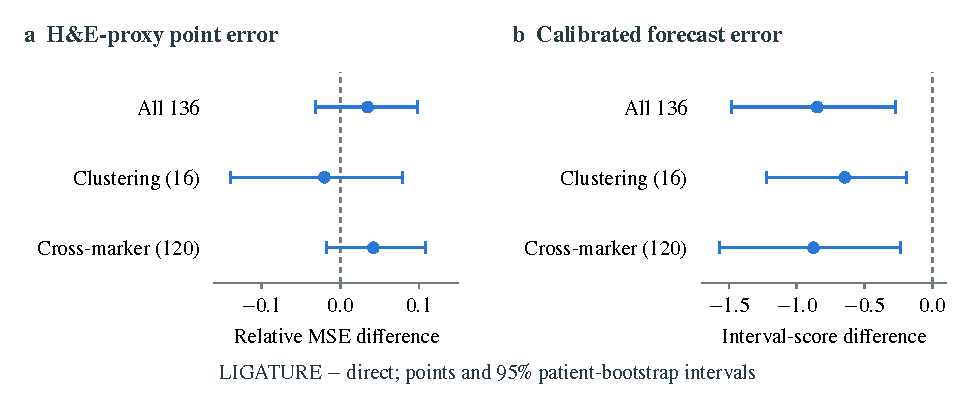
\includegraphics[width=\linewidth]{fig_geometry.pdf}
\caption{H\&E-derived nucleus-plus-rim targets: one seed, five rotations and all 40 patients. Differences are \method{} minus the matched direct graph. \textbf{a}, Point MSE in this control's own plug-in MSE units; all between-model intervals include zero. \textbf{b}, Independently calibrated 90\% interval-score differences, with overall coverage 90.6\% for both methods. Bars are conditional 95\% patient-bootstrap intervals. These targets differ from primary whole-cell targets; this is not whole-slide validation or optical-spillover correction.}
\label{fig:geometry}
\end{figure}

\begin{table}[!htp]
\centering
\caption{H\&E-derived nucleus-plus-rim targets, one seed, five rotations and all 40 patients. MSE ratios use this control's own plug-in; they are not comparable to ratios or absolute errors from a different target definition. Coverage, training-standard-deviation-normalized width and 90\% interval score summarize all 136 statistics. The direct model has lower overall point error; \method{} has lower calibrated interval score.}
\label{tab:hegeometry}

\begin{tabular}{@{}lrrrrr@{}}
\toprule
& \multicolumn{2}{c}{MSE / own plug-in} & & & \\
Method / interval & all & same & Coverage & Width & Score \\
\midrule
Plug-in / constant & 1.000 & 1.000 & 90.3\% & 4.83 & 7.18 \\
Direct / adaptive & 0.925 & 0.721 & 90.6\% & 4.70 & 6.96 \\
Direct / constant & 0.925 & 0.721 & 90.3\% & 4.66 & 6.94 \\
\method{} / adaptive & 0.960 & 0.701 & 90.6\% & 4.46 & 6.11 \\
\method{} / constant & 0.960 & 0.701 & 90.8\% & 4.70 & 6.89 \\
\bottomrule
\end{tabular}

\end{table}

\end{document}
